\section{Unified Control-Theoretic Training}

\begin{frame}{Content Overview}
    \footnotesize
    \begin{enumerate}
        \item \textcolor{gray!50}{Introduction, Background, and Objectives}
        \item \textcolor{gray!50}{Addressing the Impossible Trinity of Modeling (ITM)}
        \item \colorbox{yellow!70}{\textbf{Unified Control-Theoretic Training}}
        \item \textcolor{gray!50}{Addressing the Impossible Trinity of Optimal Control (ITOC)}
        \item \textcolor{gray!50}{Conclusions and Future Work}
    \end{enumerate}
\end{frame}

\begin{frame}{Unified Control-Theoretic Training}
    
    {\huge\textbf{Second Contribution}}
    {\footnotesize
    \begin{itemize}
        \item Unified control-theoretic view for physics-infused ROMs and closed-loop optimal control
    \end{itemize}}

\end{frame}

\begin{frame}{Unified Control-Theoretic Training: NODE to Generalized Framework}
    \footnotesize
    \visible<1->{\textbf{We step back} from NODE-like training and consider an \textbf{optimal-control-theoretic} perspective,}
    \only<2>{
        \begin{figure}
            \vspace*{-0.05in}
            \centering
            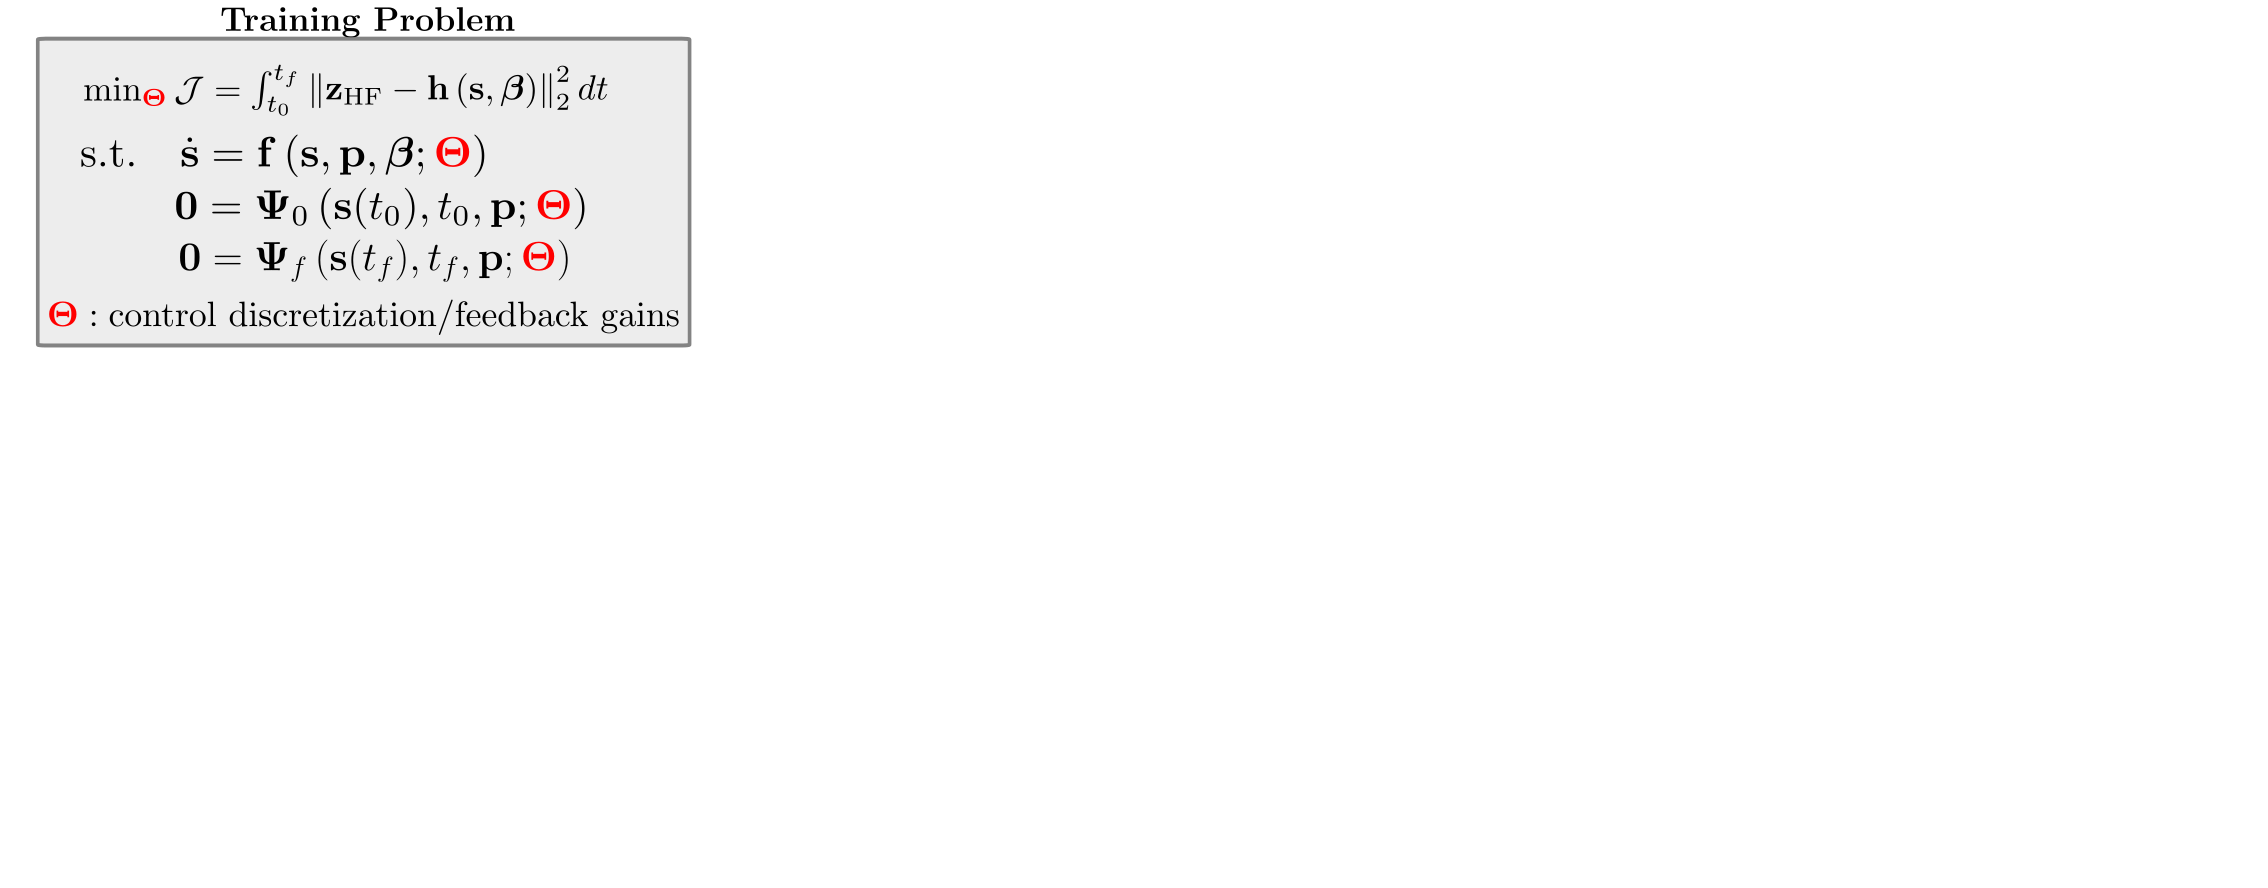
\includegraphics[width=0.95\textwidth]{../figs/ct/ct_overview_1.png}
        \end{figure}}
    \only<3>{
        \begin{figure}
            \centering
            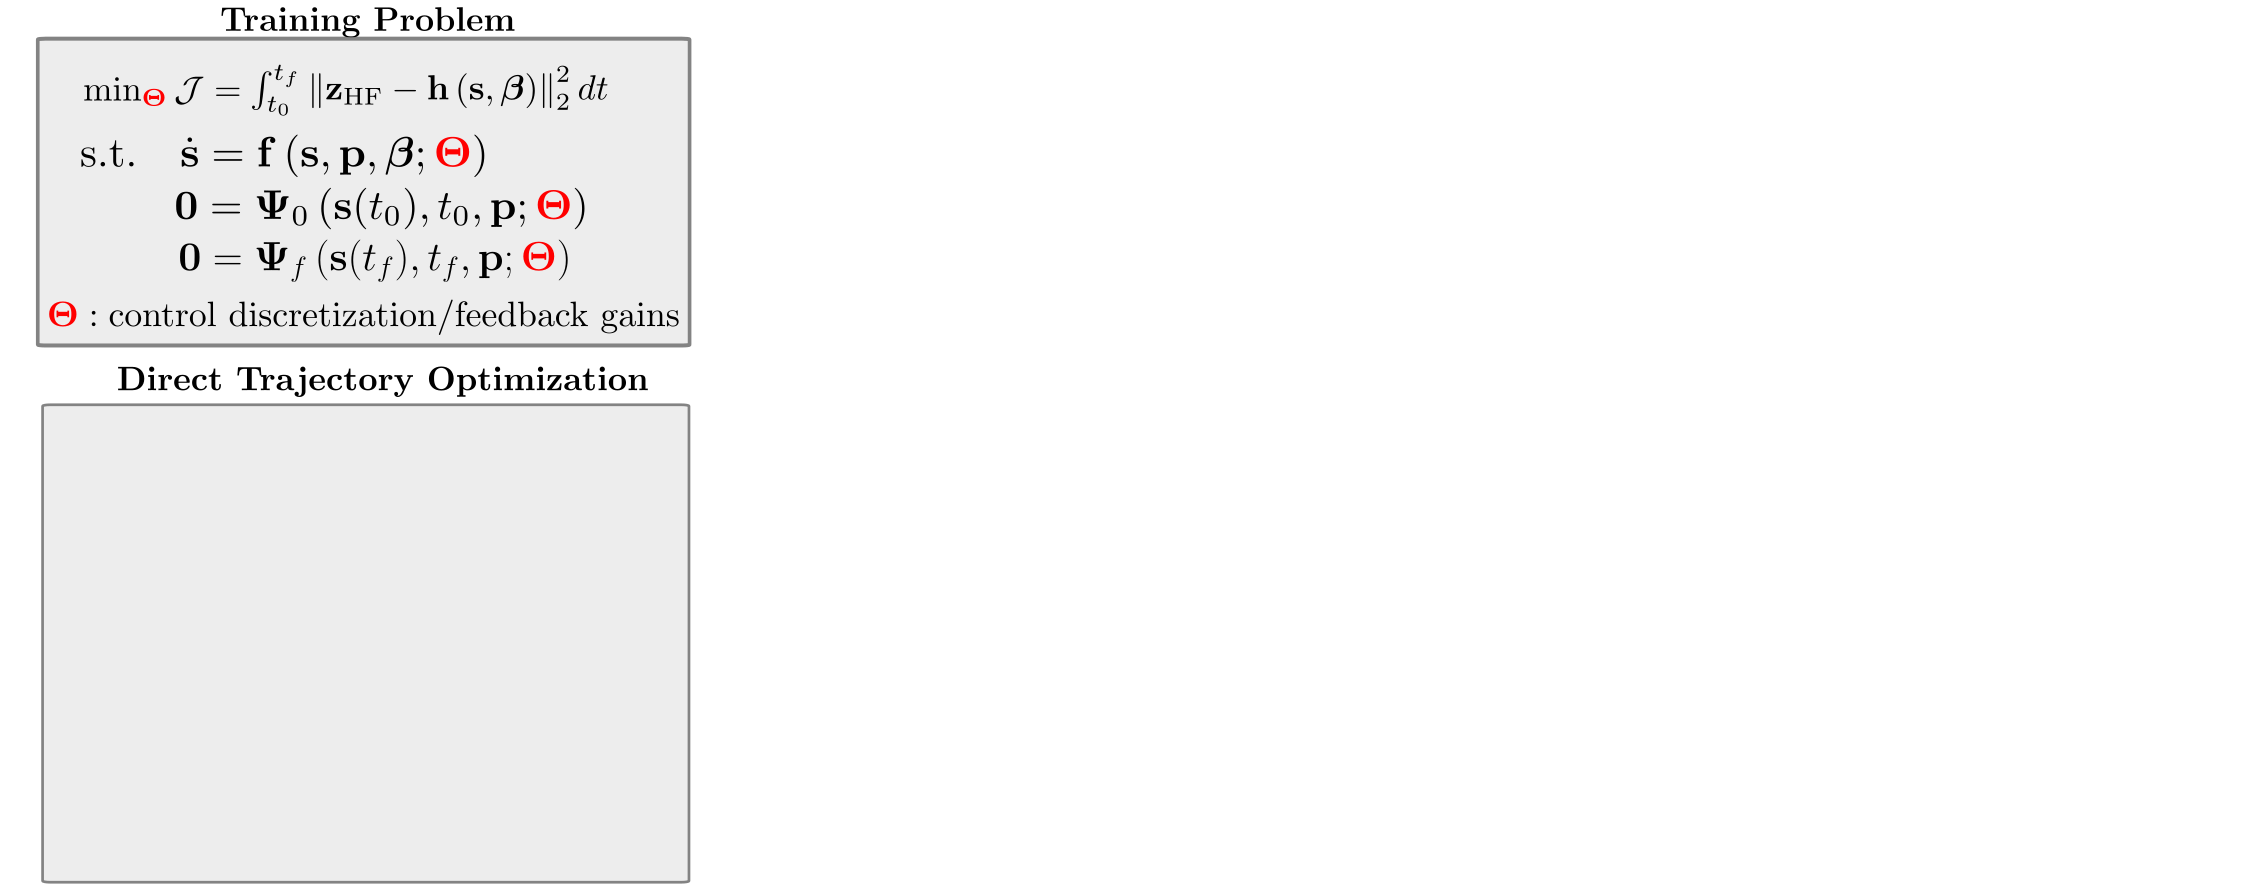
\includegraphics[width=0.95\textwidth]{../figs/ct/ct_overview_2.png}
        \end{figure}}
    \only<4>{
        \begin{figure}
            \centering
            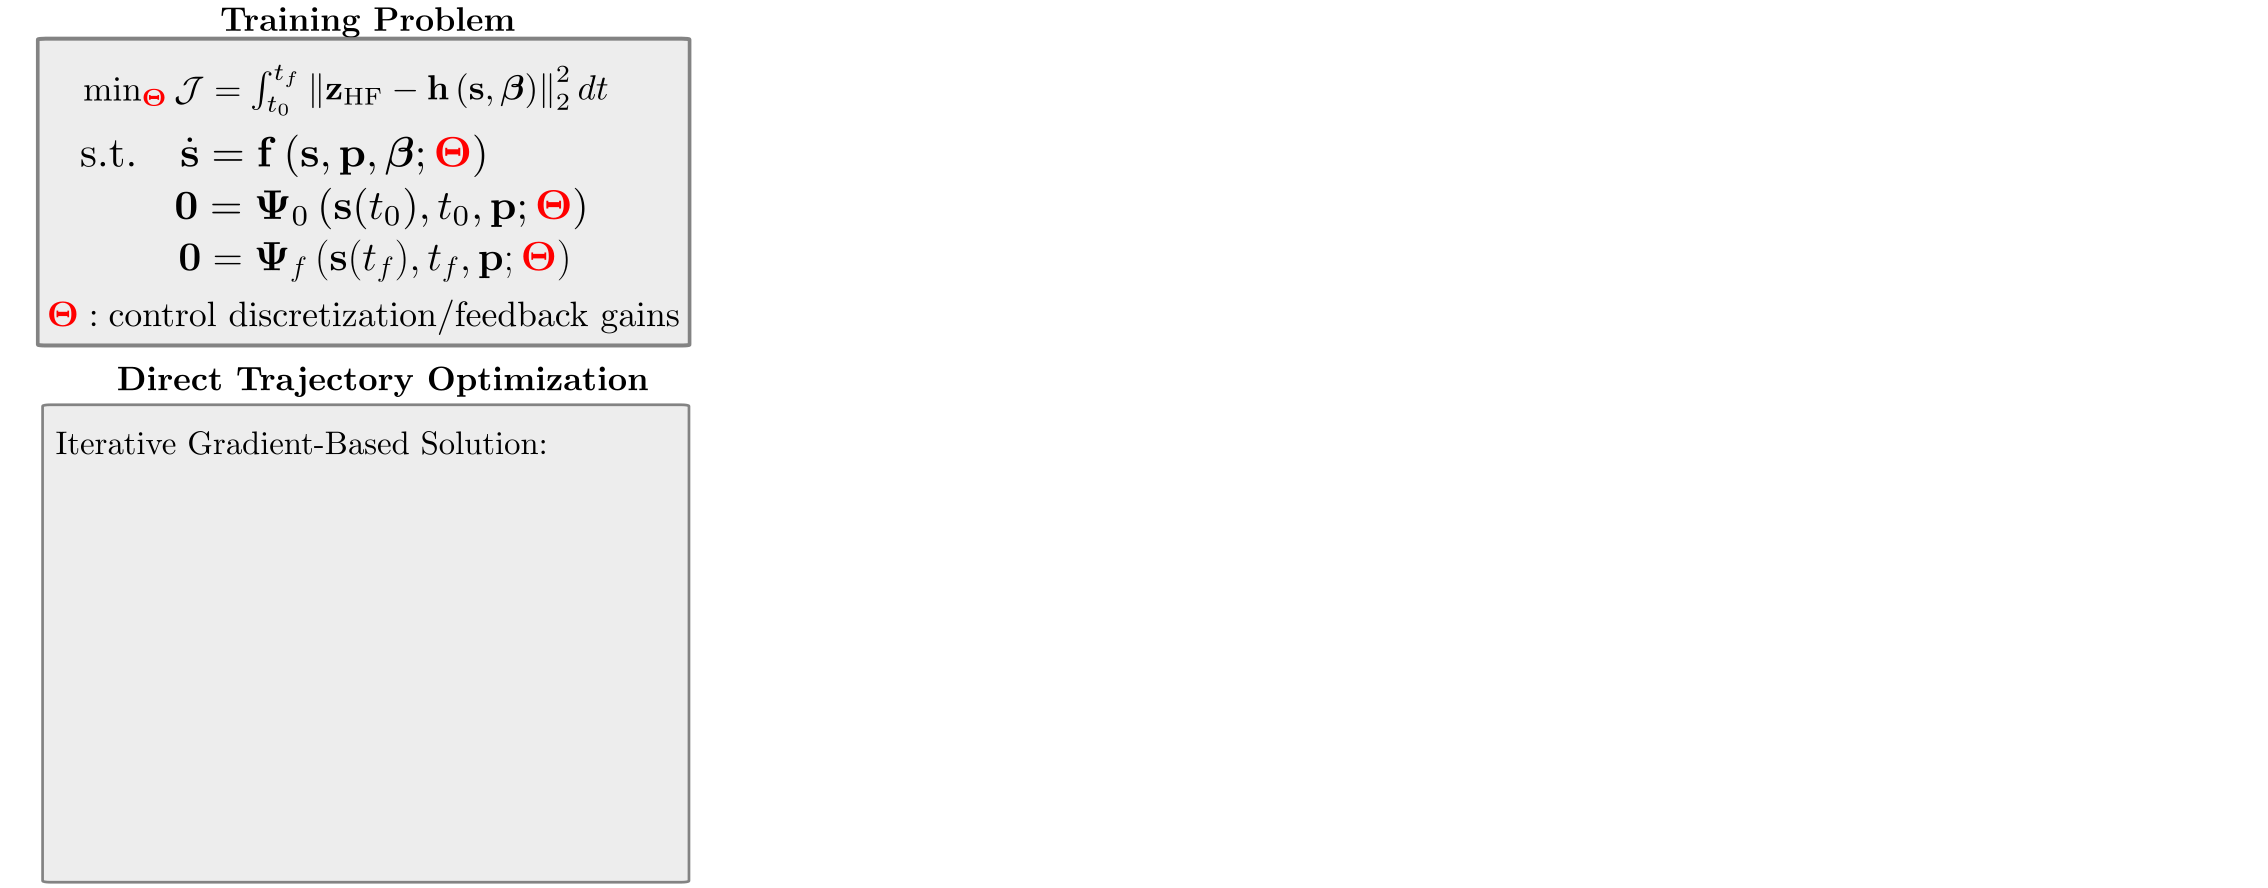
\includegraphics[width=0.95\textwidth]{../figs/ct/ct_overview_3.png}
        \end{figure}}
    \only<5>{
        \begin{figure}
            \centering
            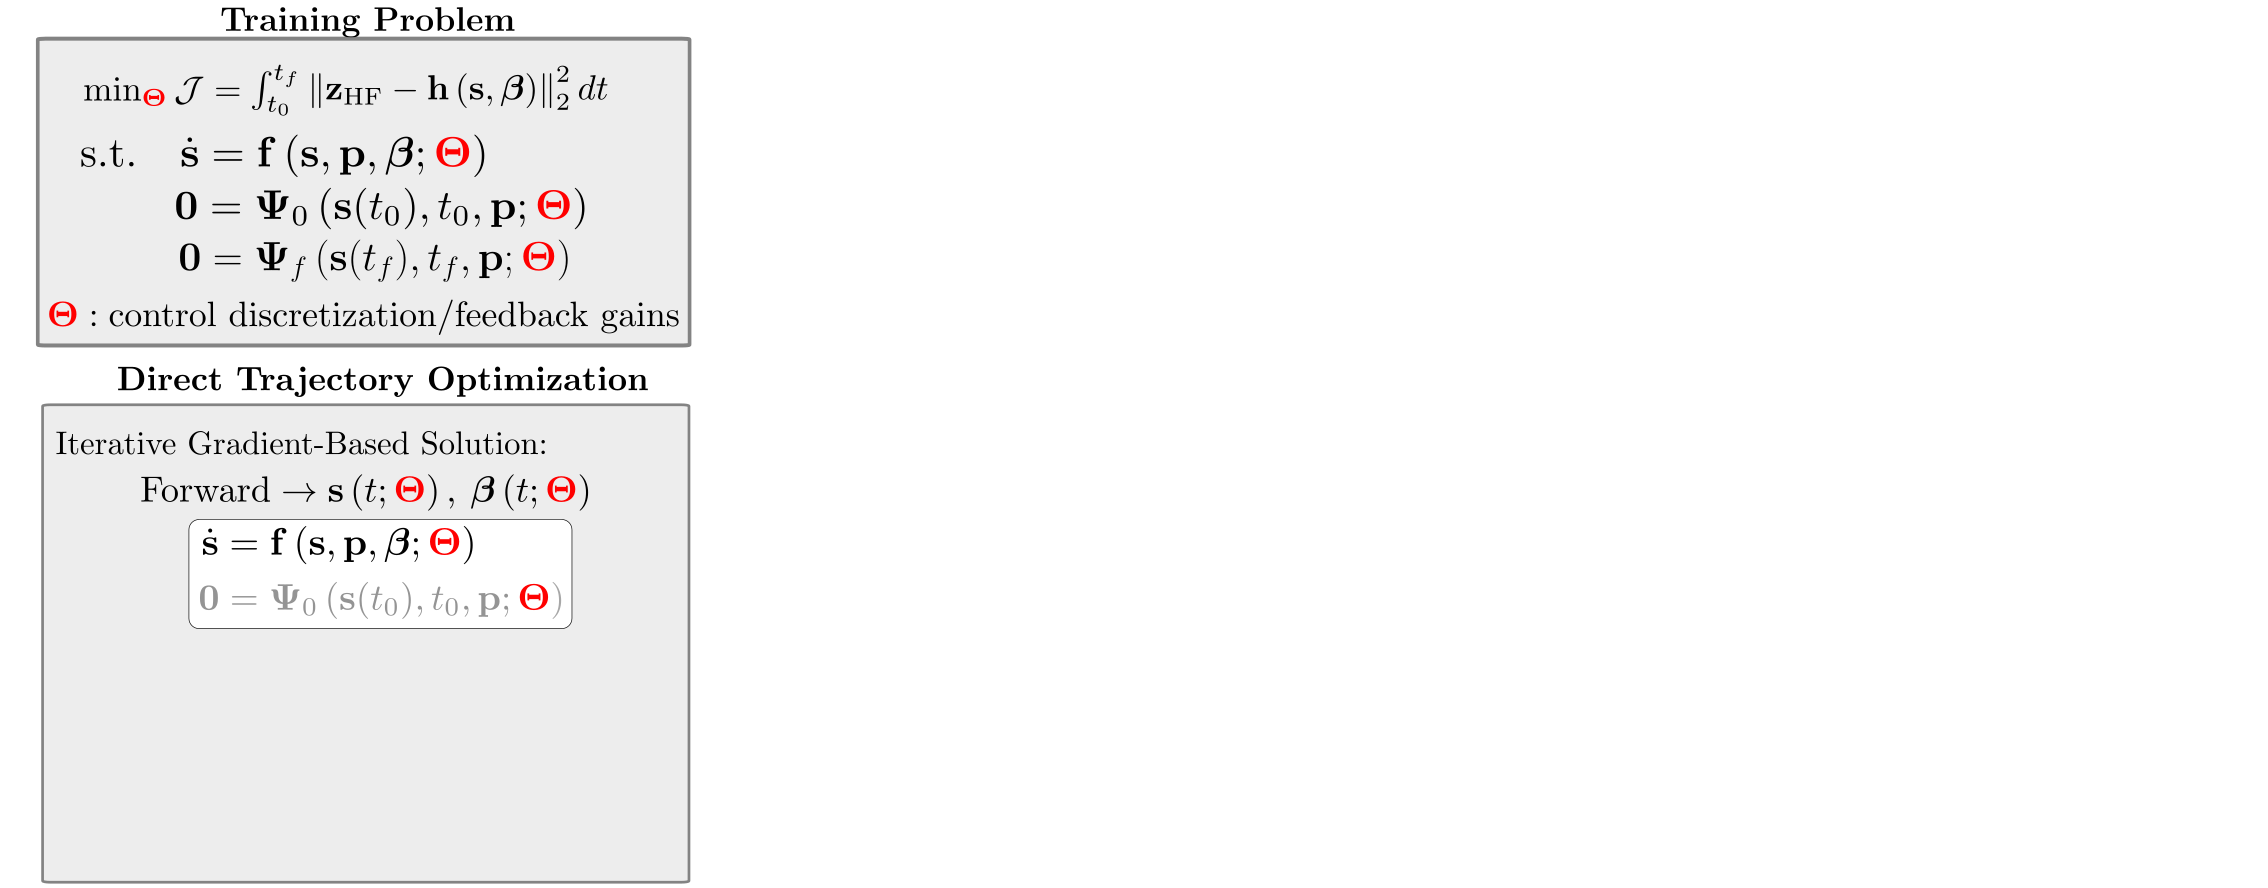
\includegraphics[width=0.95\textwidth]{../figs/ct/ct_overview_4.png}
        \end{figure}}
    \only<6>{
        \begin{figure}
            \centering
            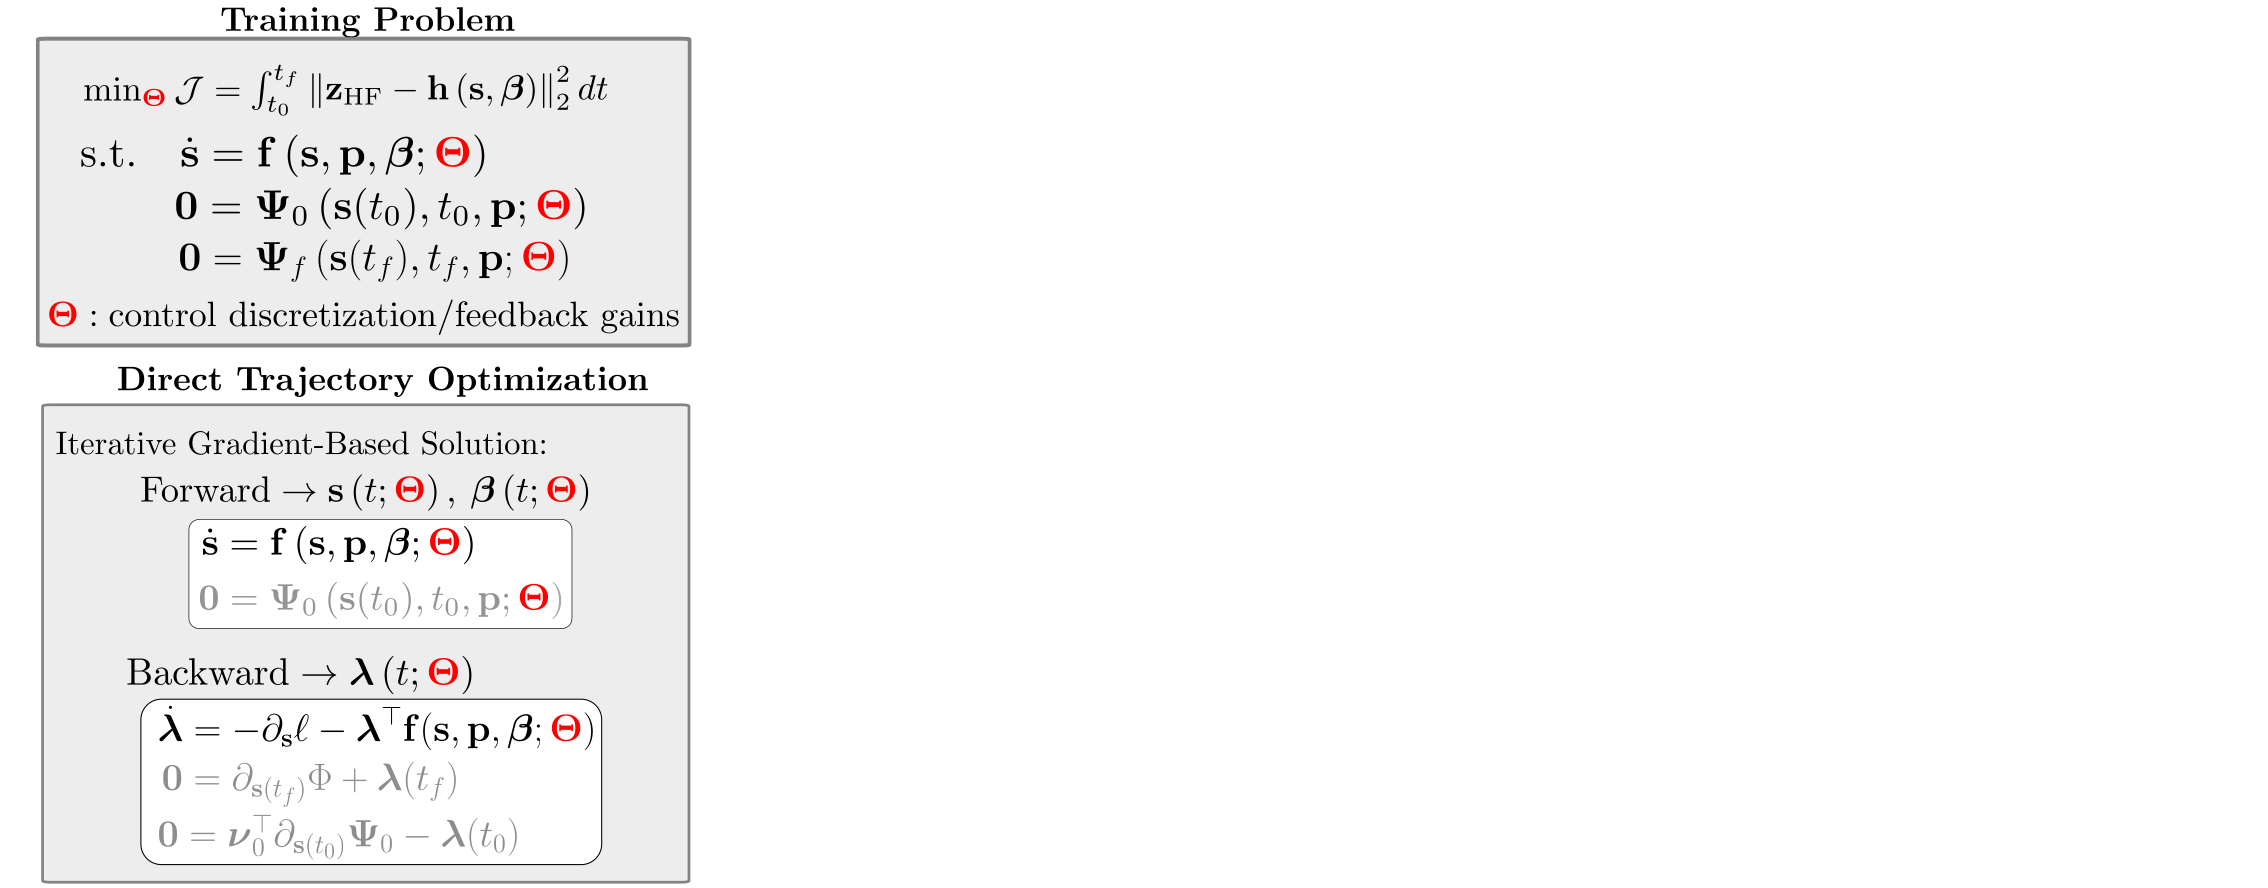
\includegraphics[width=0.95\textwidth]{../figs/ct/ct_overview_5.png}
        \end{figure}}
    \only<7>{
        \begin{figure}
            \centering
            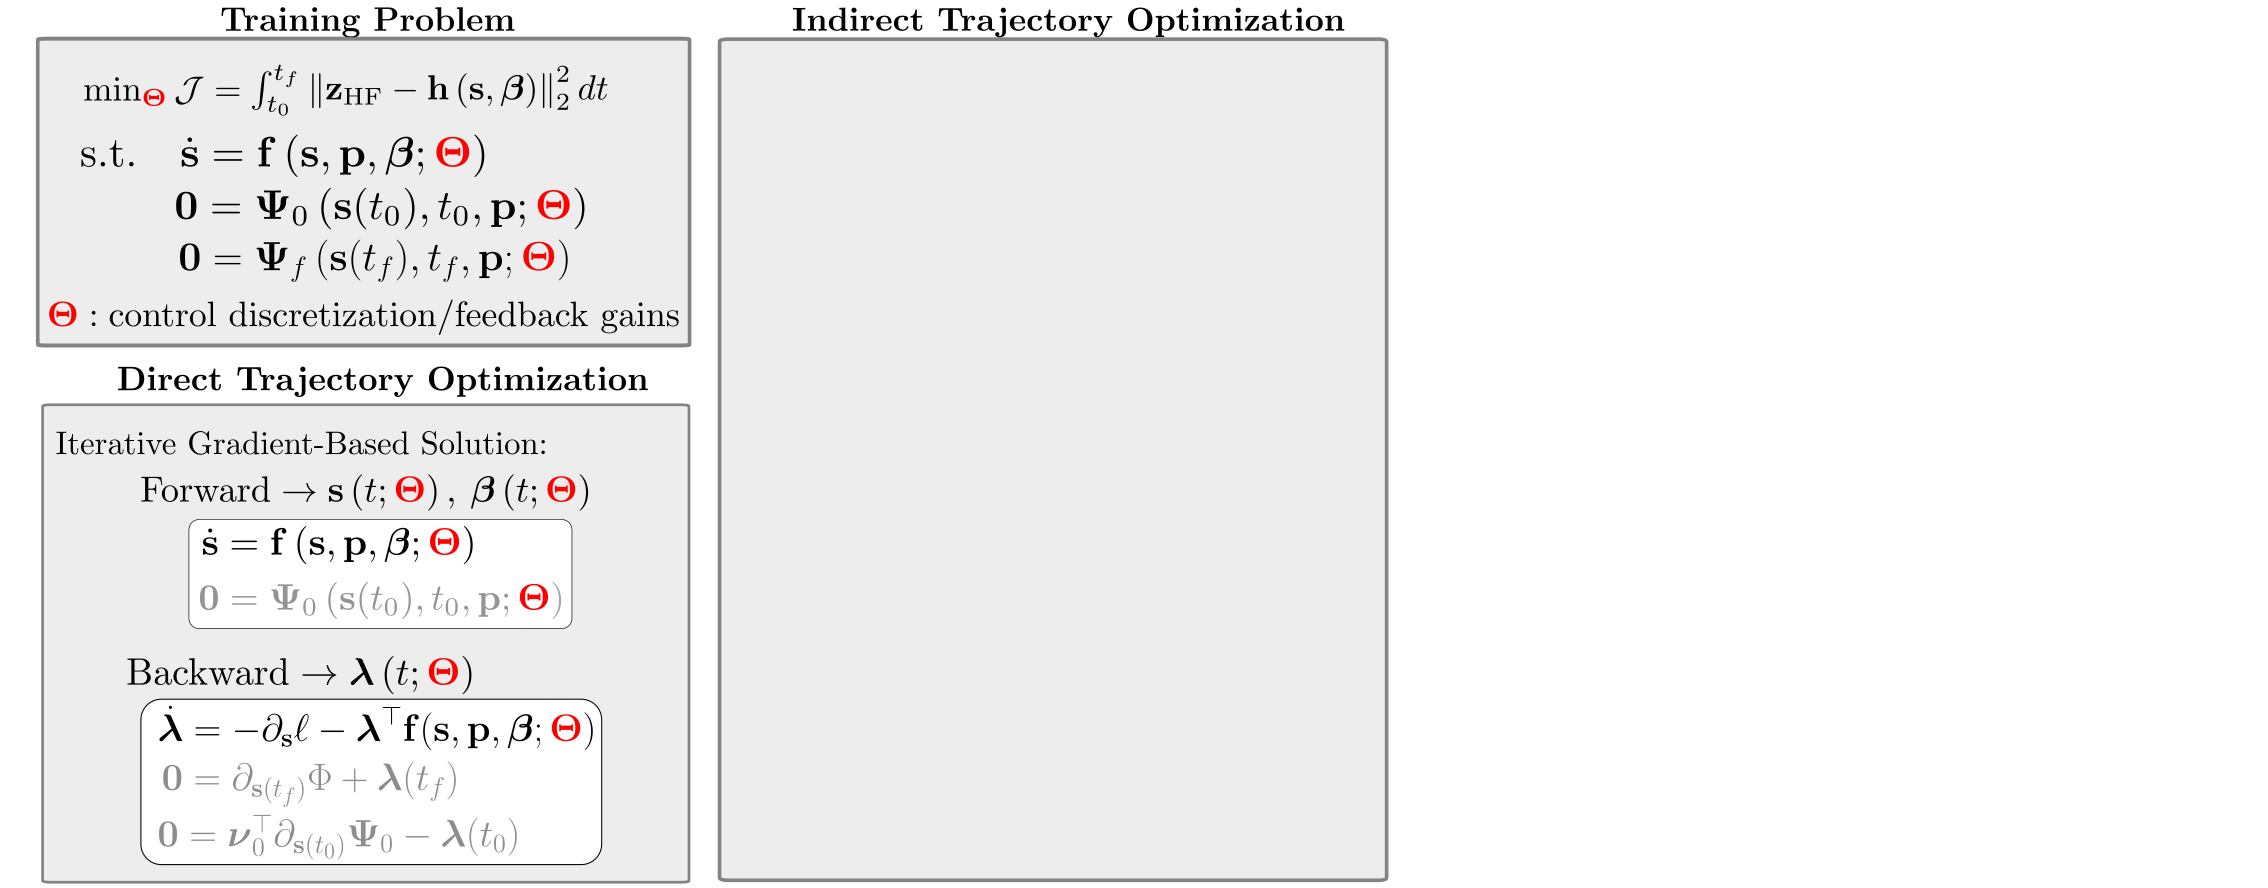
\includegraphics[width=0.95\textwidth]{../figs/ct/ct_overview_6.png}
        \end{figure}}
    \only<8>{
        \begin{figure}
            \centering
            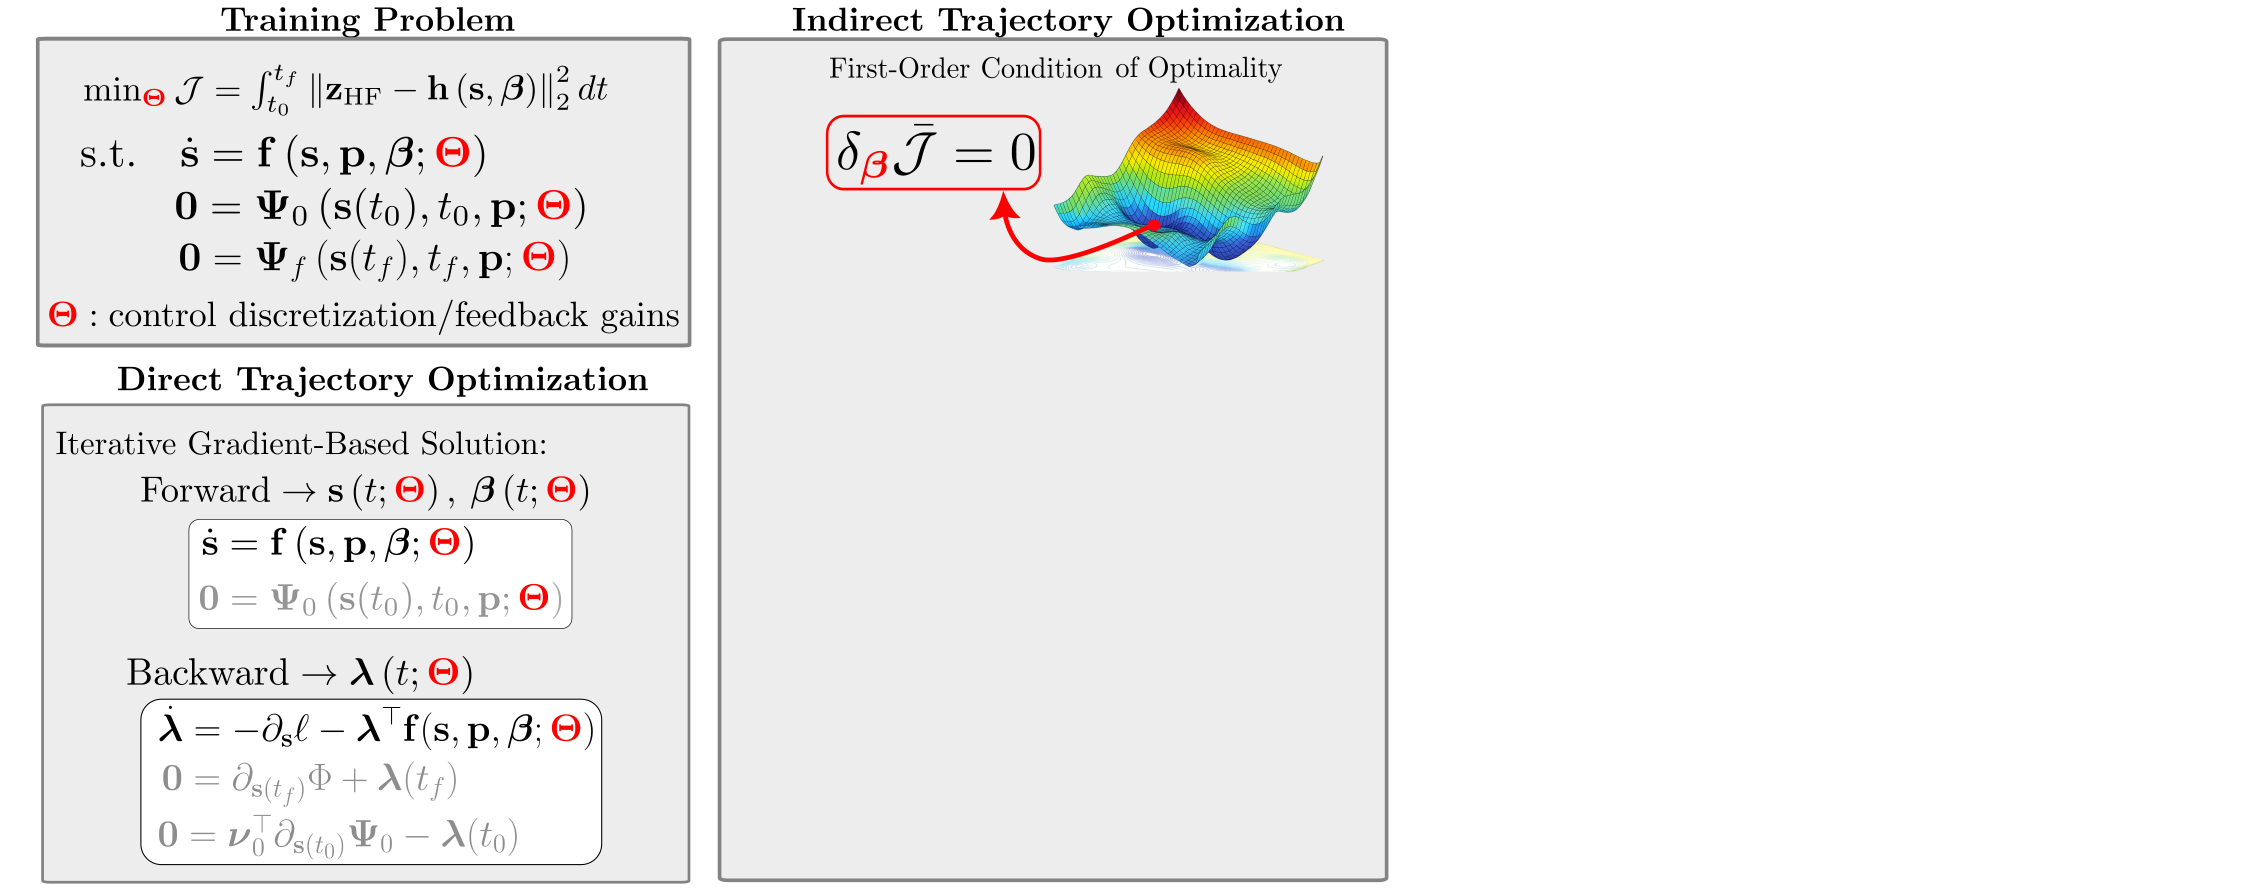
\includegraphics[width=0.95\textwidth]{../figs/ct/ct_overview_7.png}
        \end{figure}}
    \only<9>{
        \begin{figure}
            \centering
            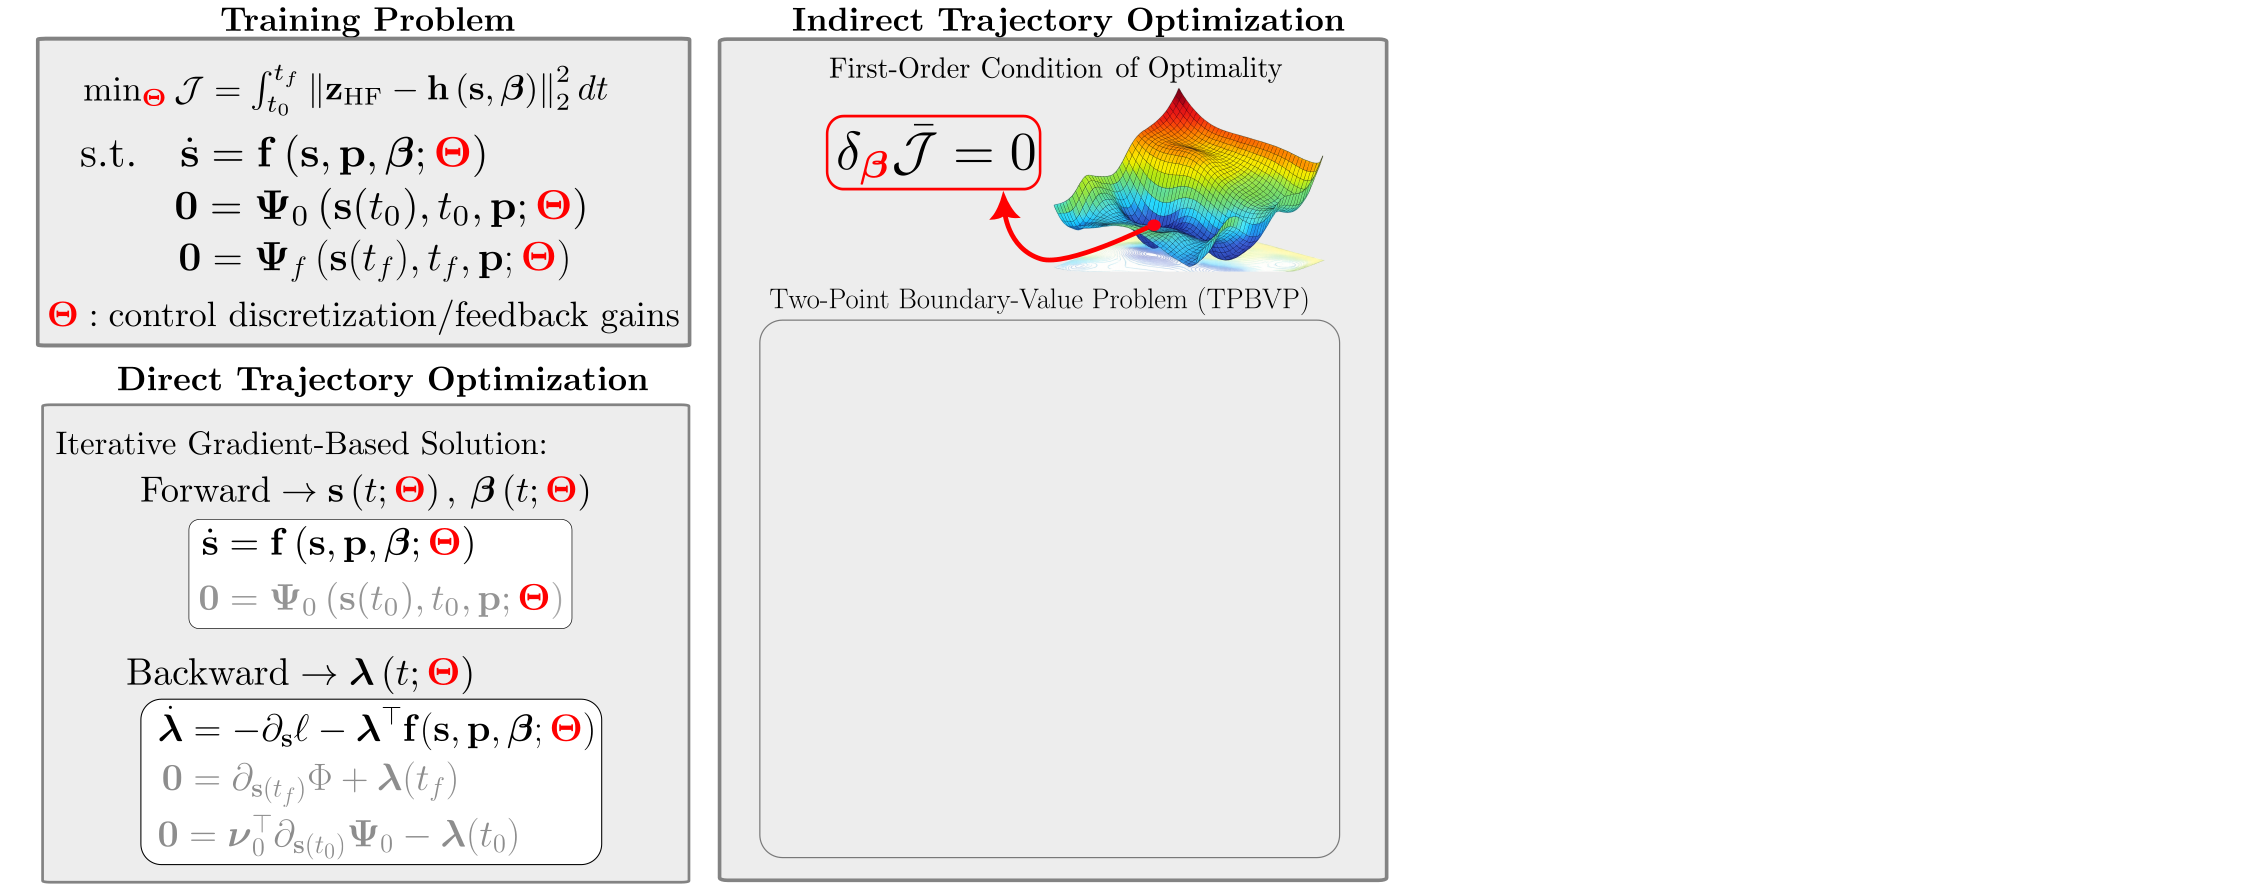
\includegraphics[width=0.95\textwidth]{../figs/ct/ct_overview_8.png}
        \end{figure}}
    \only<10>{
        \begin{figure}
            \centering
            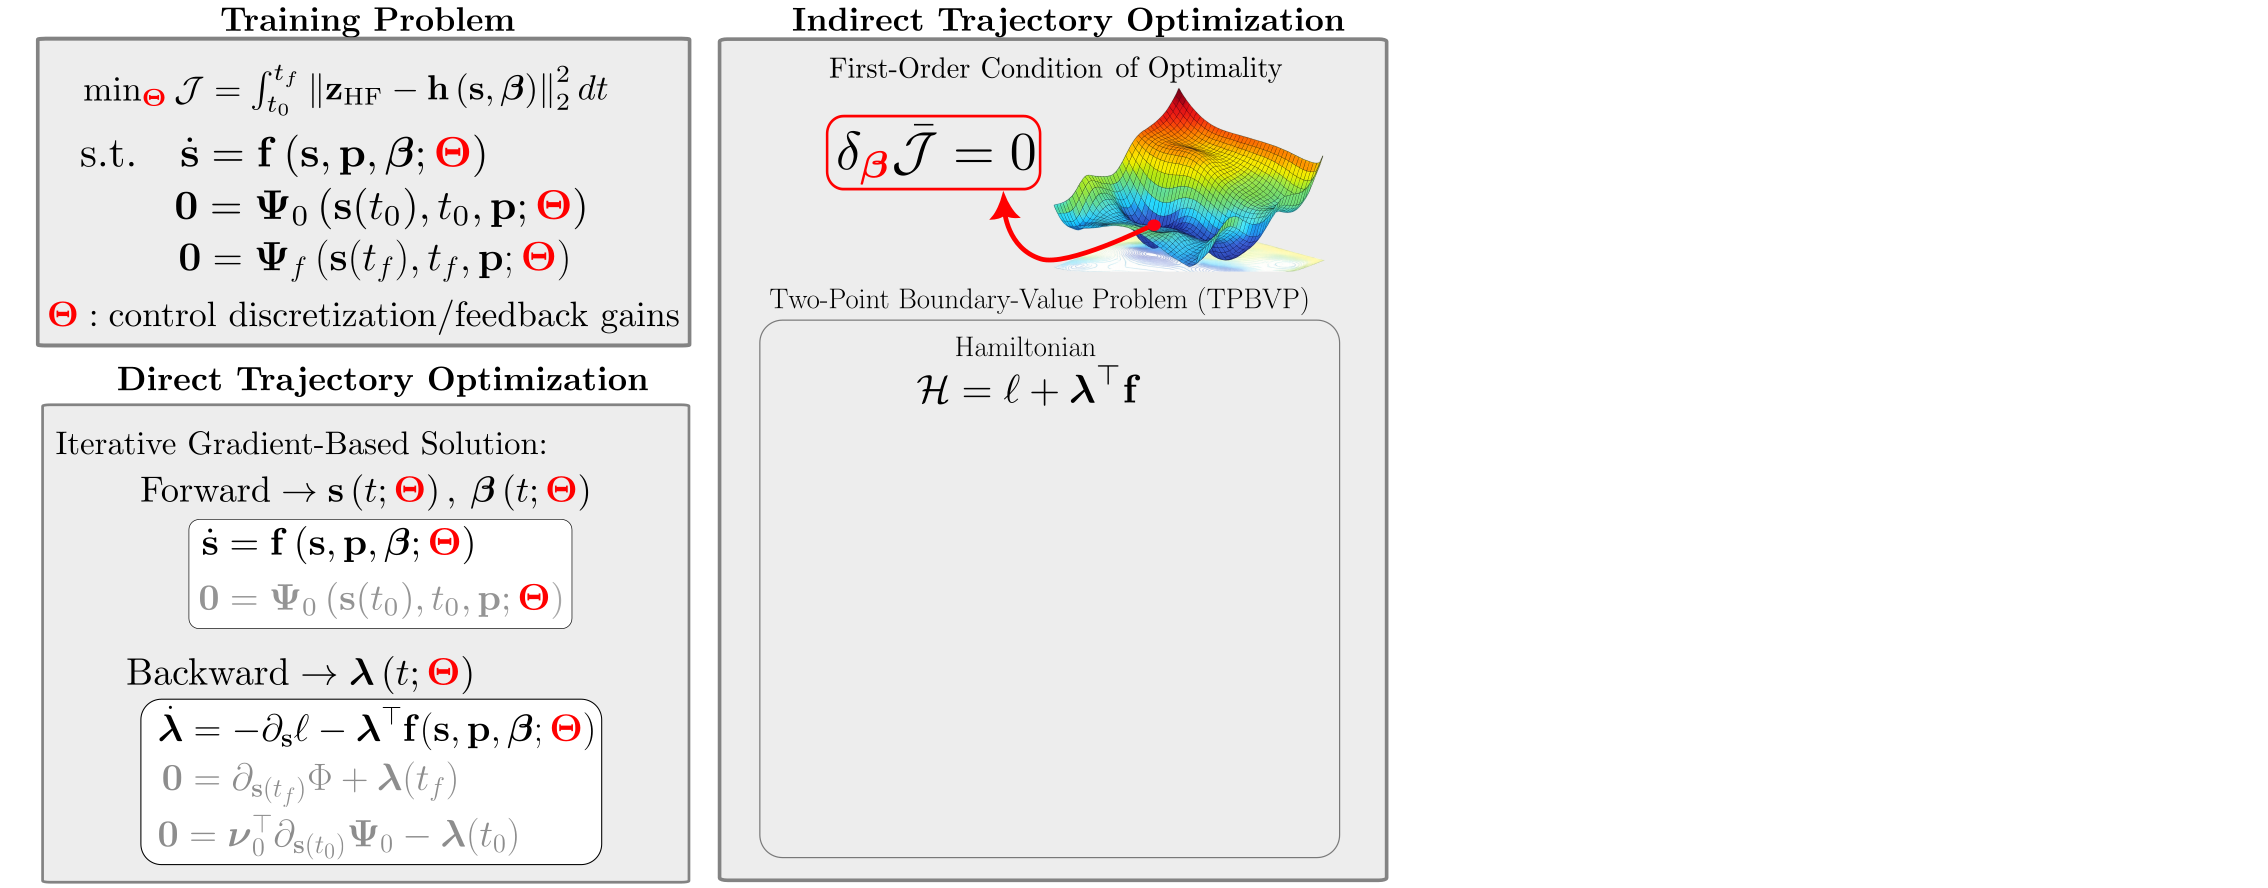
\includegraphics[width=0.95\textwidth]{../figs/ct/ct_overview_9.png}
        \end{figure}}
    \only<11>{
        \begin{figure}
            \centering
            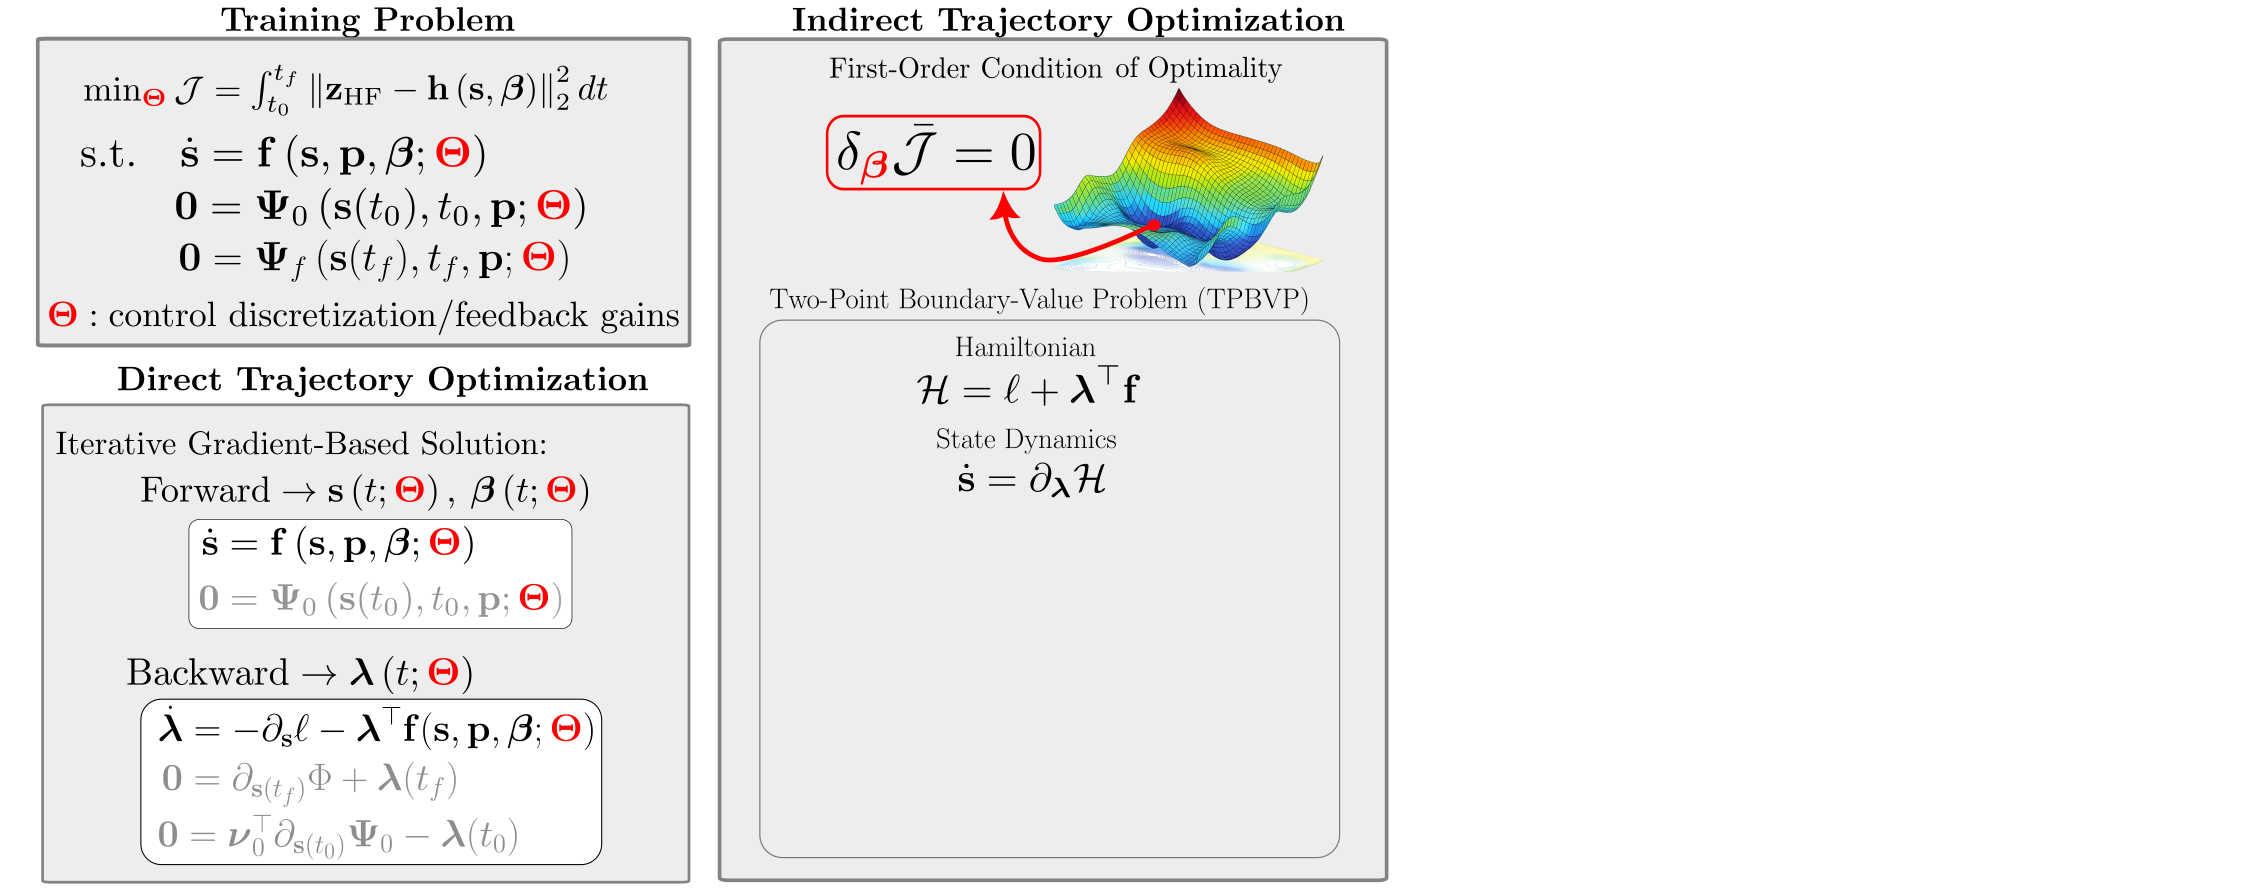
\includegraphics[width=0.95\textwidth]{../figs/ct/ct_overview_10.png}
        \end{figure}}
    \only<12>{
        \begin{figure}
            \centering
            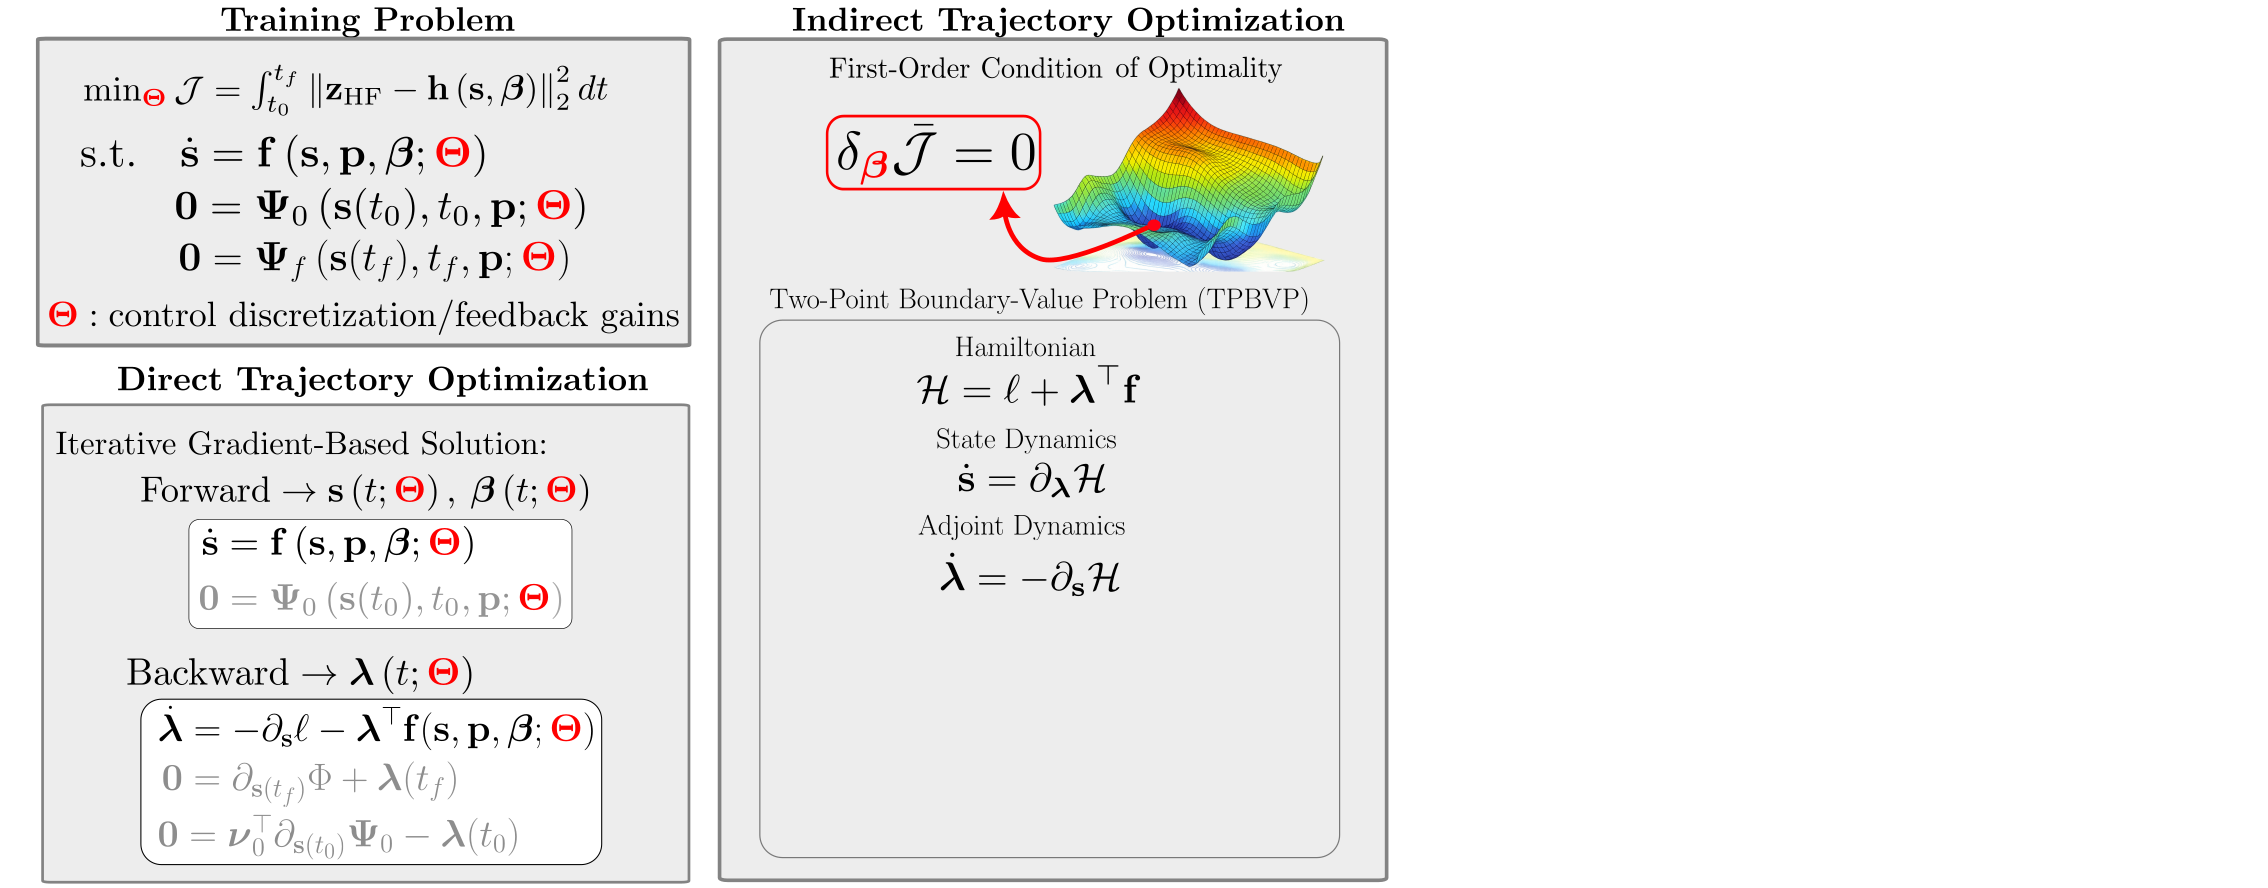
\includegraphics[width=0.95\textwidth]{../figs/ct/ct_overview_11.png}
        \end{figure}}
    \only<13>{
        \begin{figure}
            \centering
            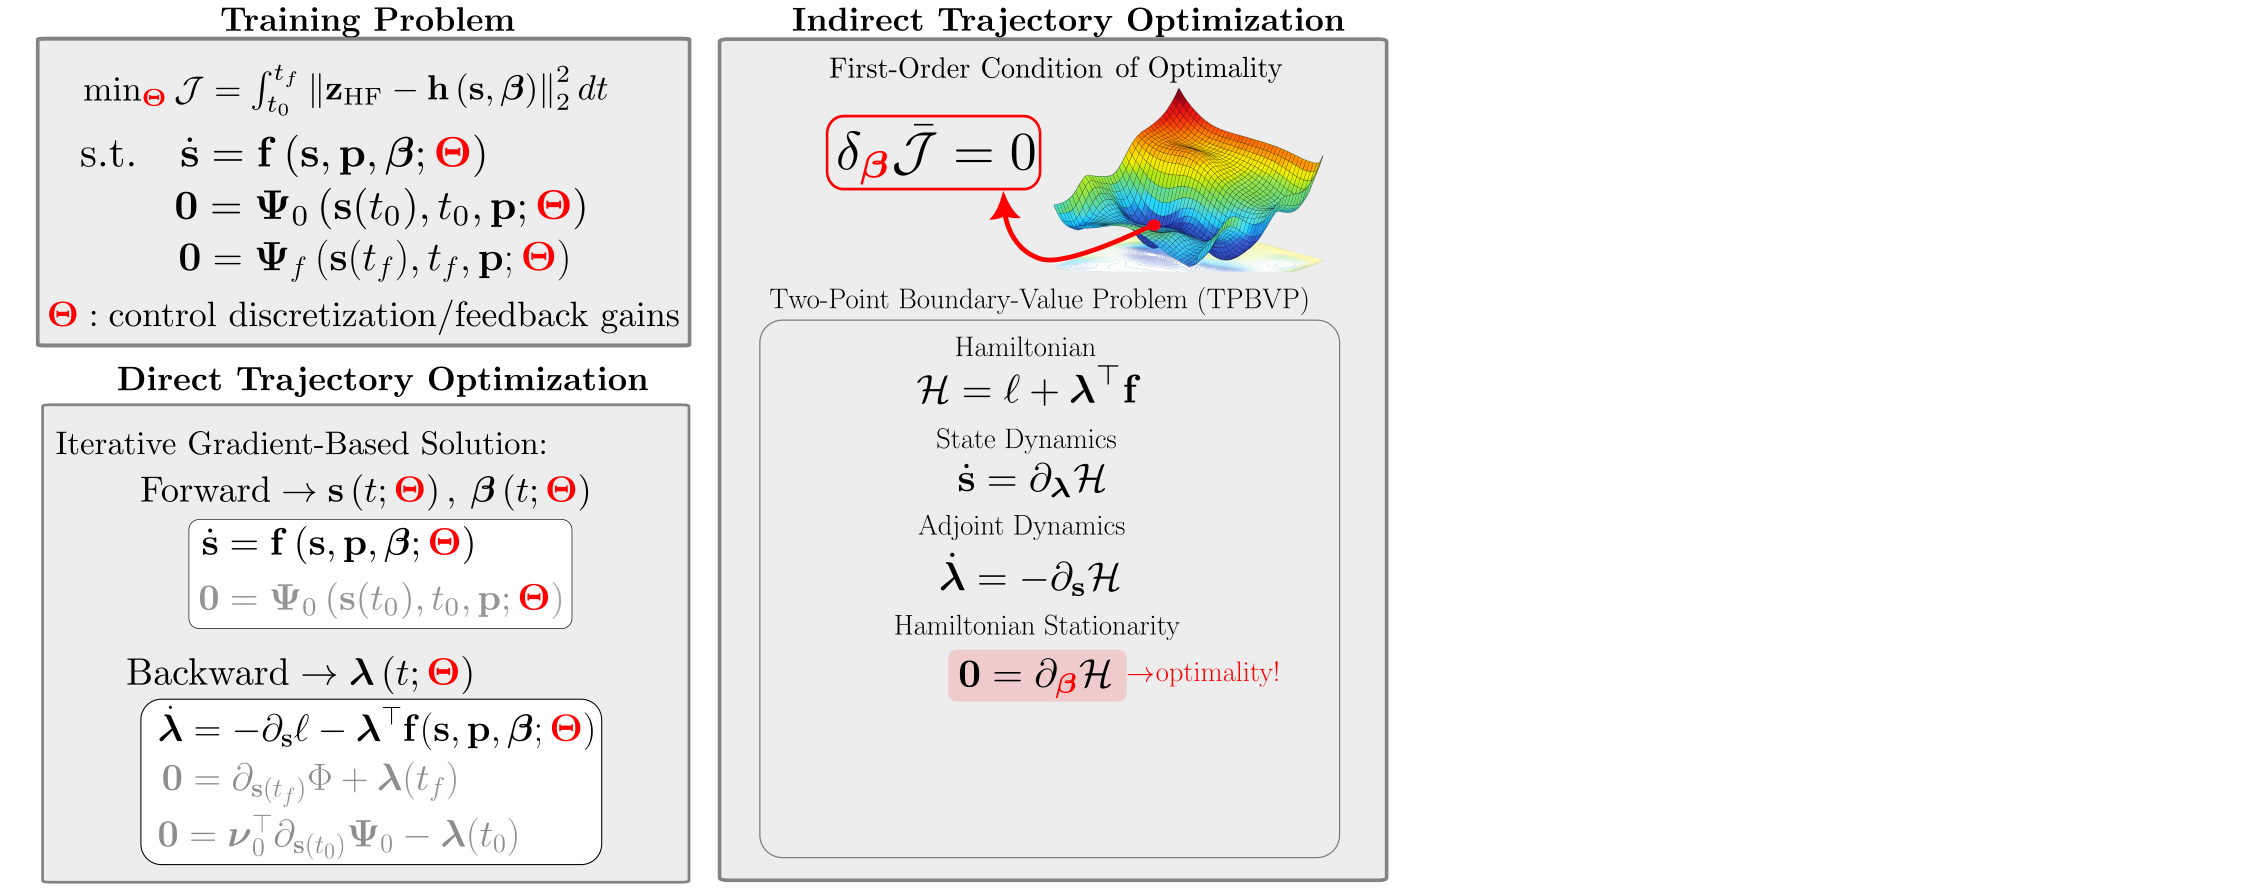
\includegraphics[width=0.95\textwidth]{../figs/ct/ct_overview_12.png}
        \end{figure}}
    \only<14>{
        \begin{figure}
            \centering
            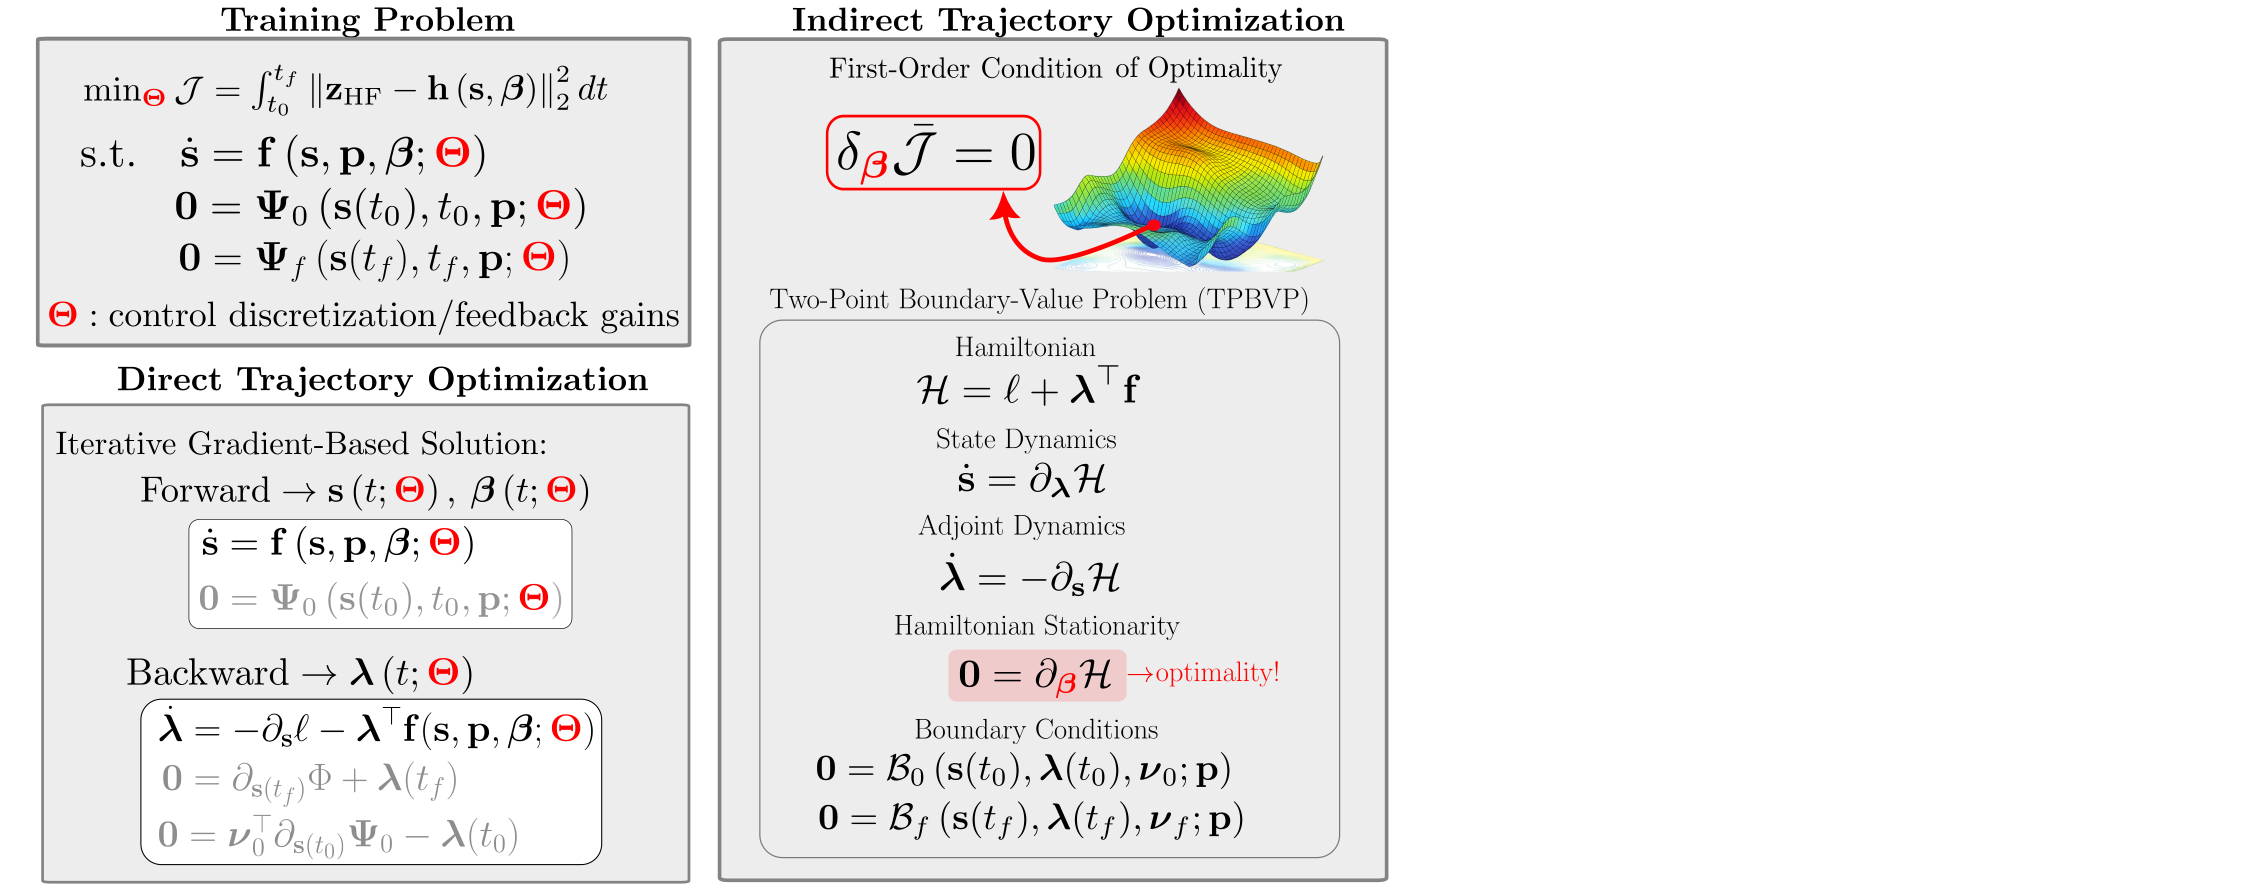
\includegraphics[width=0.95\textwidth]{../figs/ct/ct_overview_13.png}
        \end{figure}}
    \only<15>{
        \begin{figure}
            \centering
            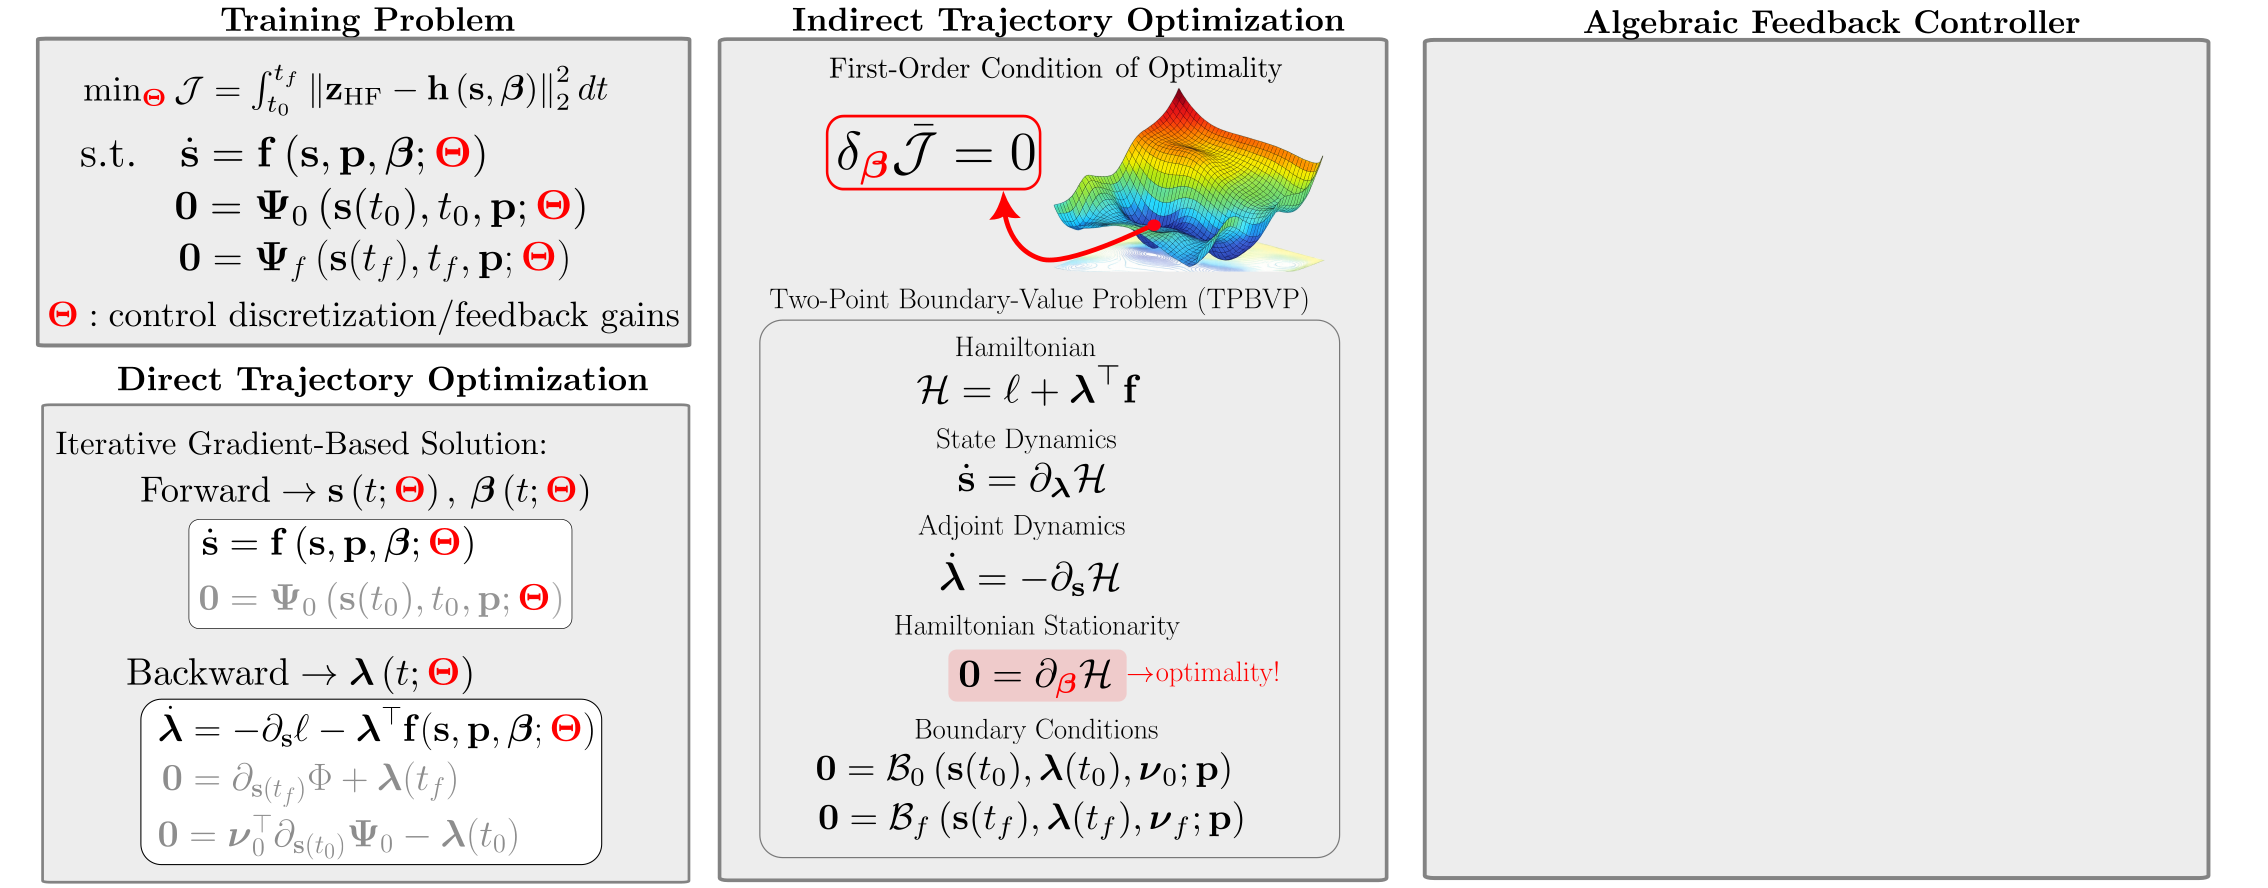
\includegraphics[width=0.95\textwidth]{../figs/ct/ct_overview_14.png}
        \end{figure}}
    \only<16>{
        \begin{figure}
            \centering
            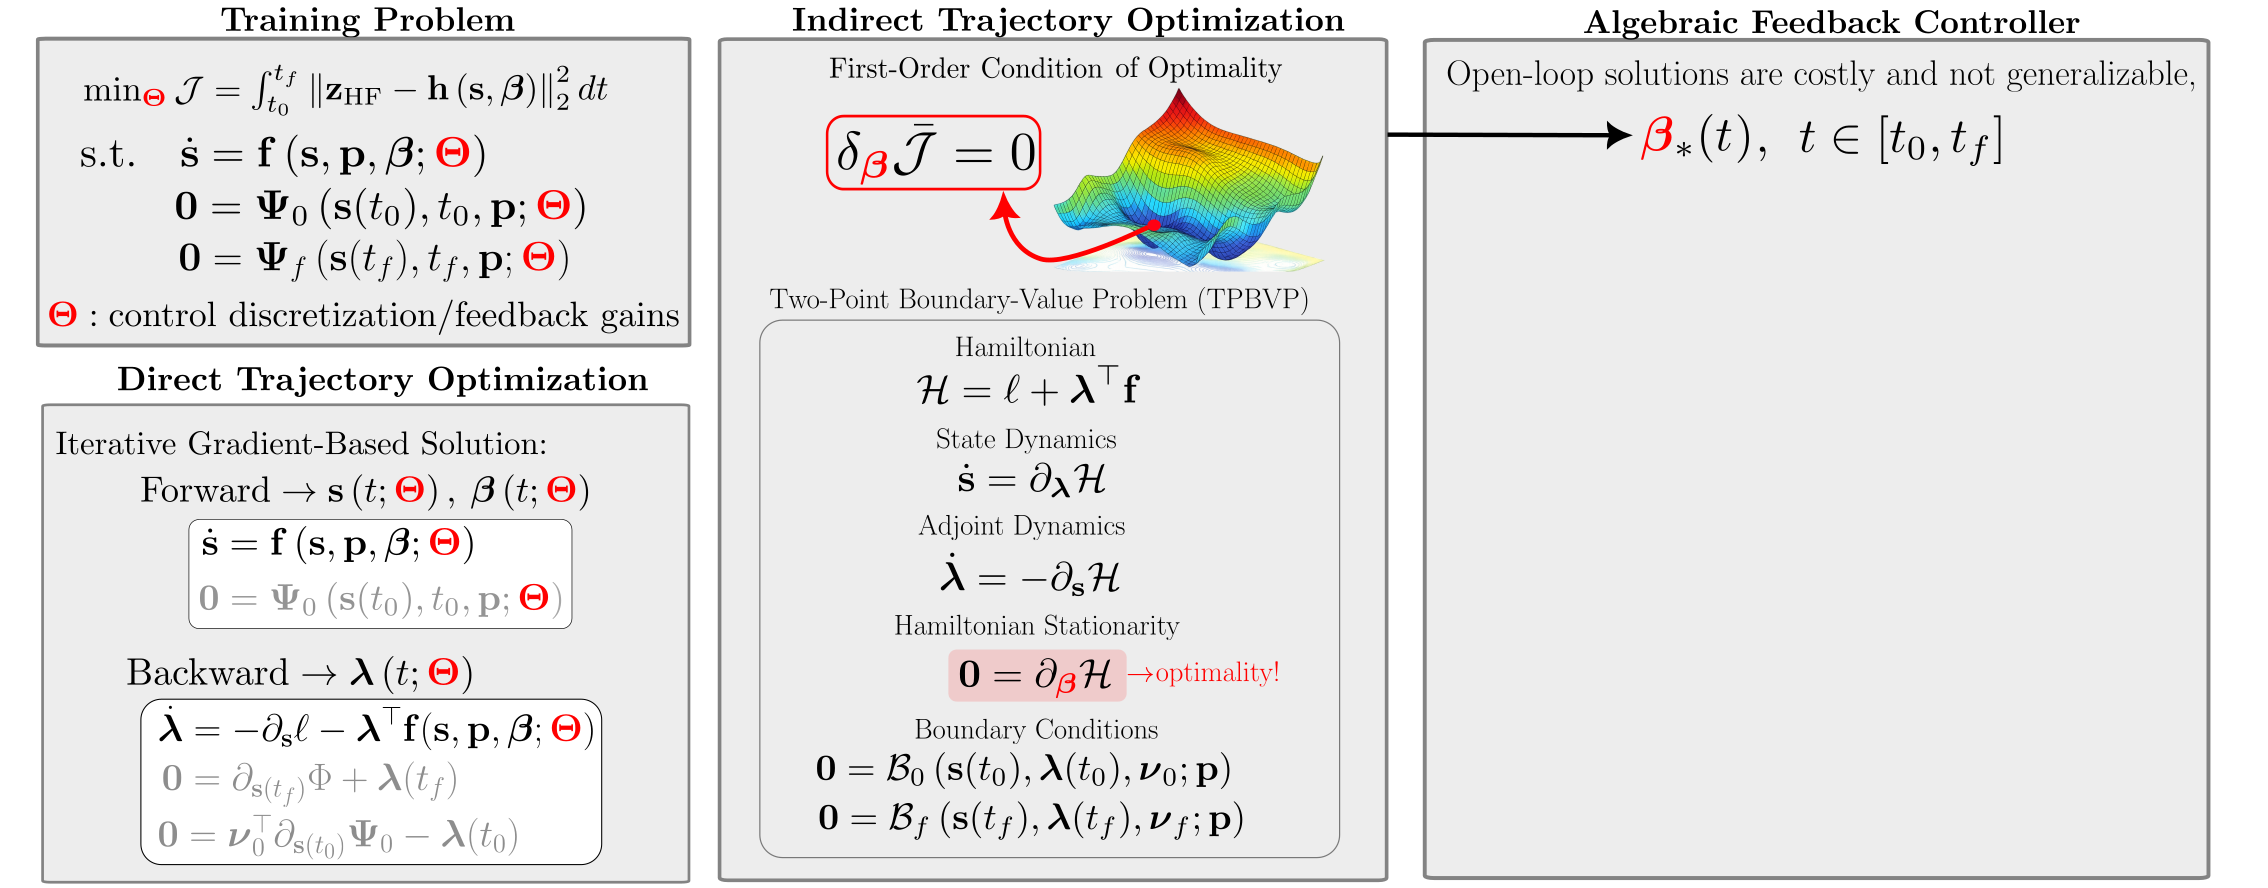
\includegraphics[width=0.95\textwidth]{../figs/ct/ct_overview_15.png}
        \end{figure}}
    \only<17>{
        \begin{figure}
            \centering
            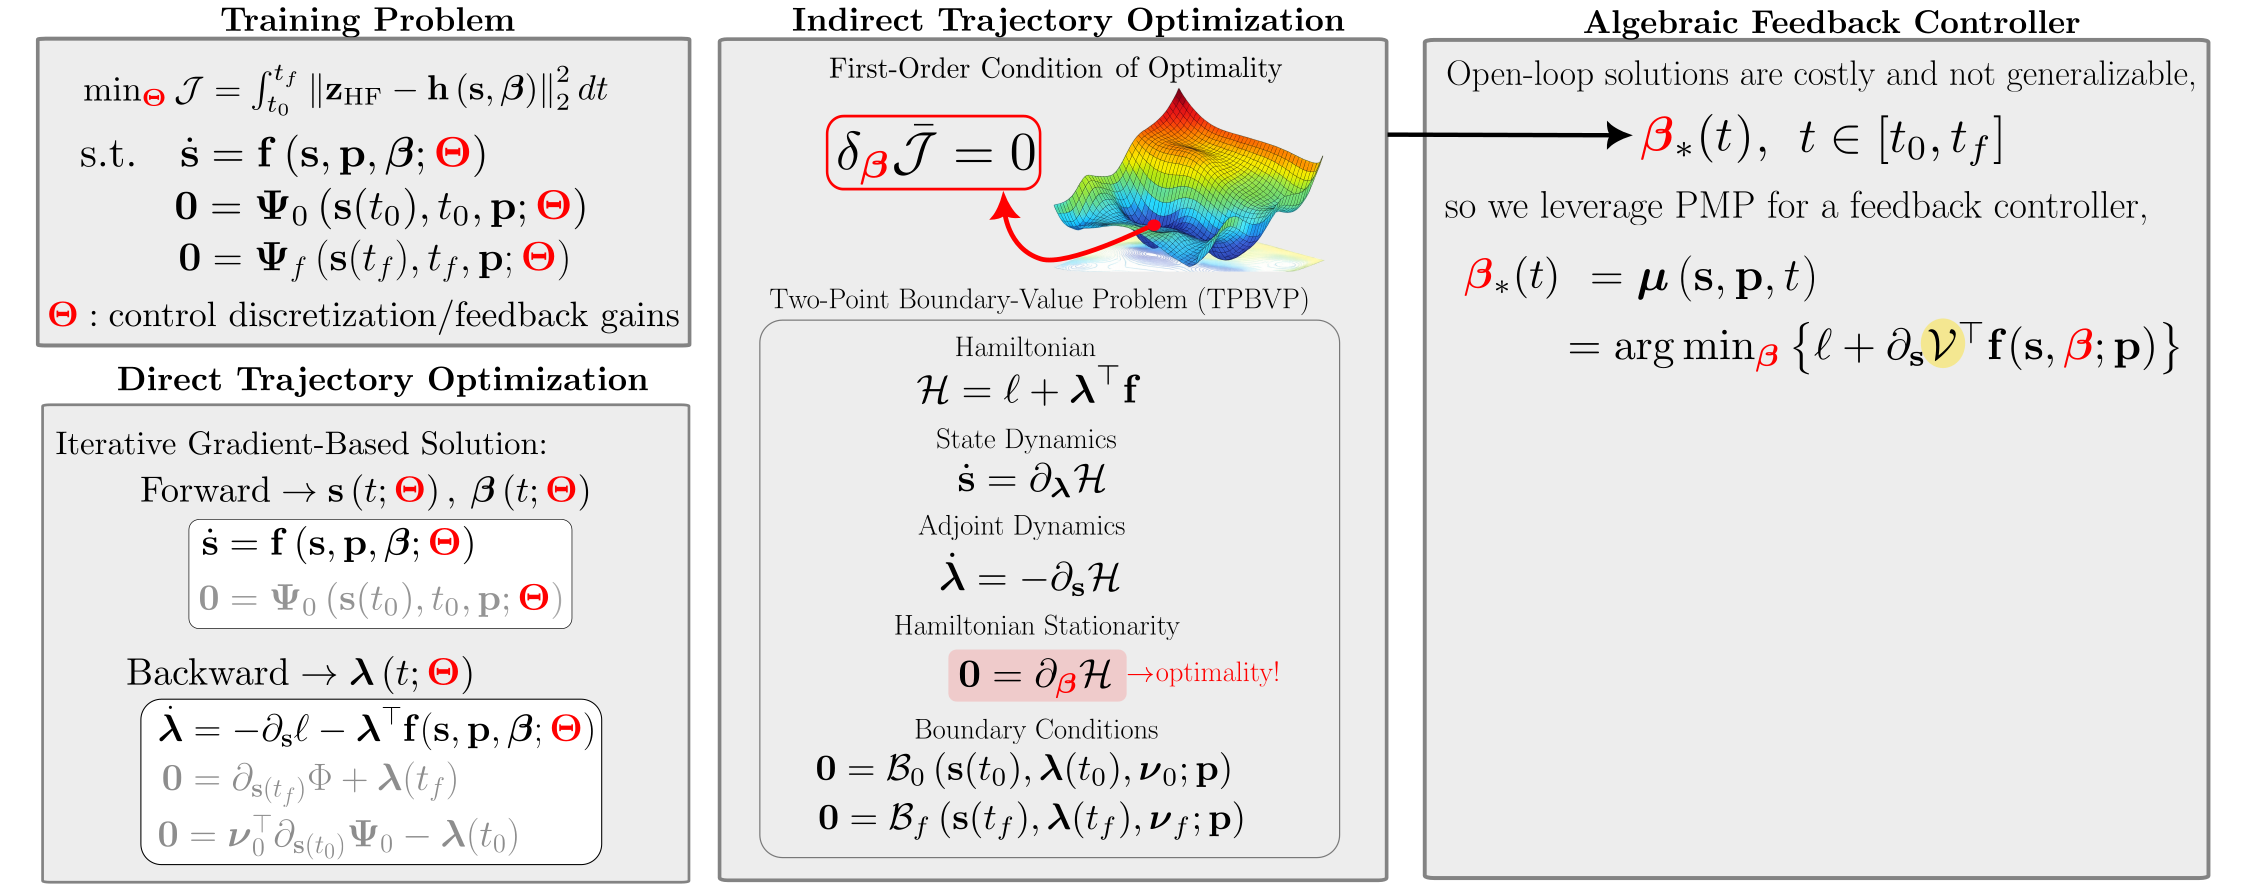
\includegraphics[width=0.95\textwidth]{../figs/ct/ct_overview_16.png}
        \end{figure}}
    \only<18>{
        \begin{figure}
            \centering
            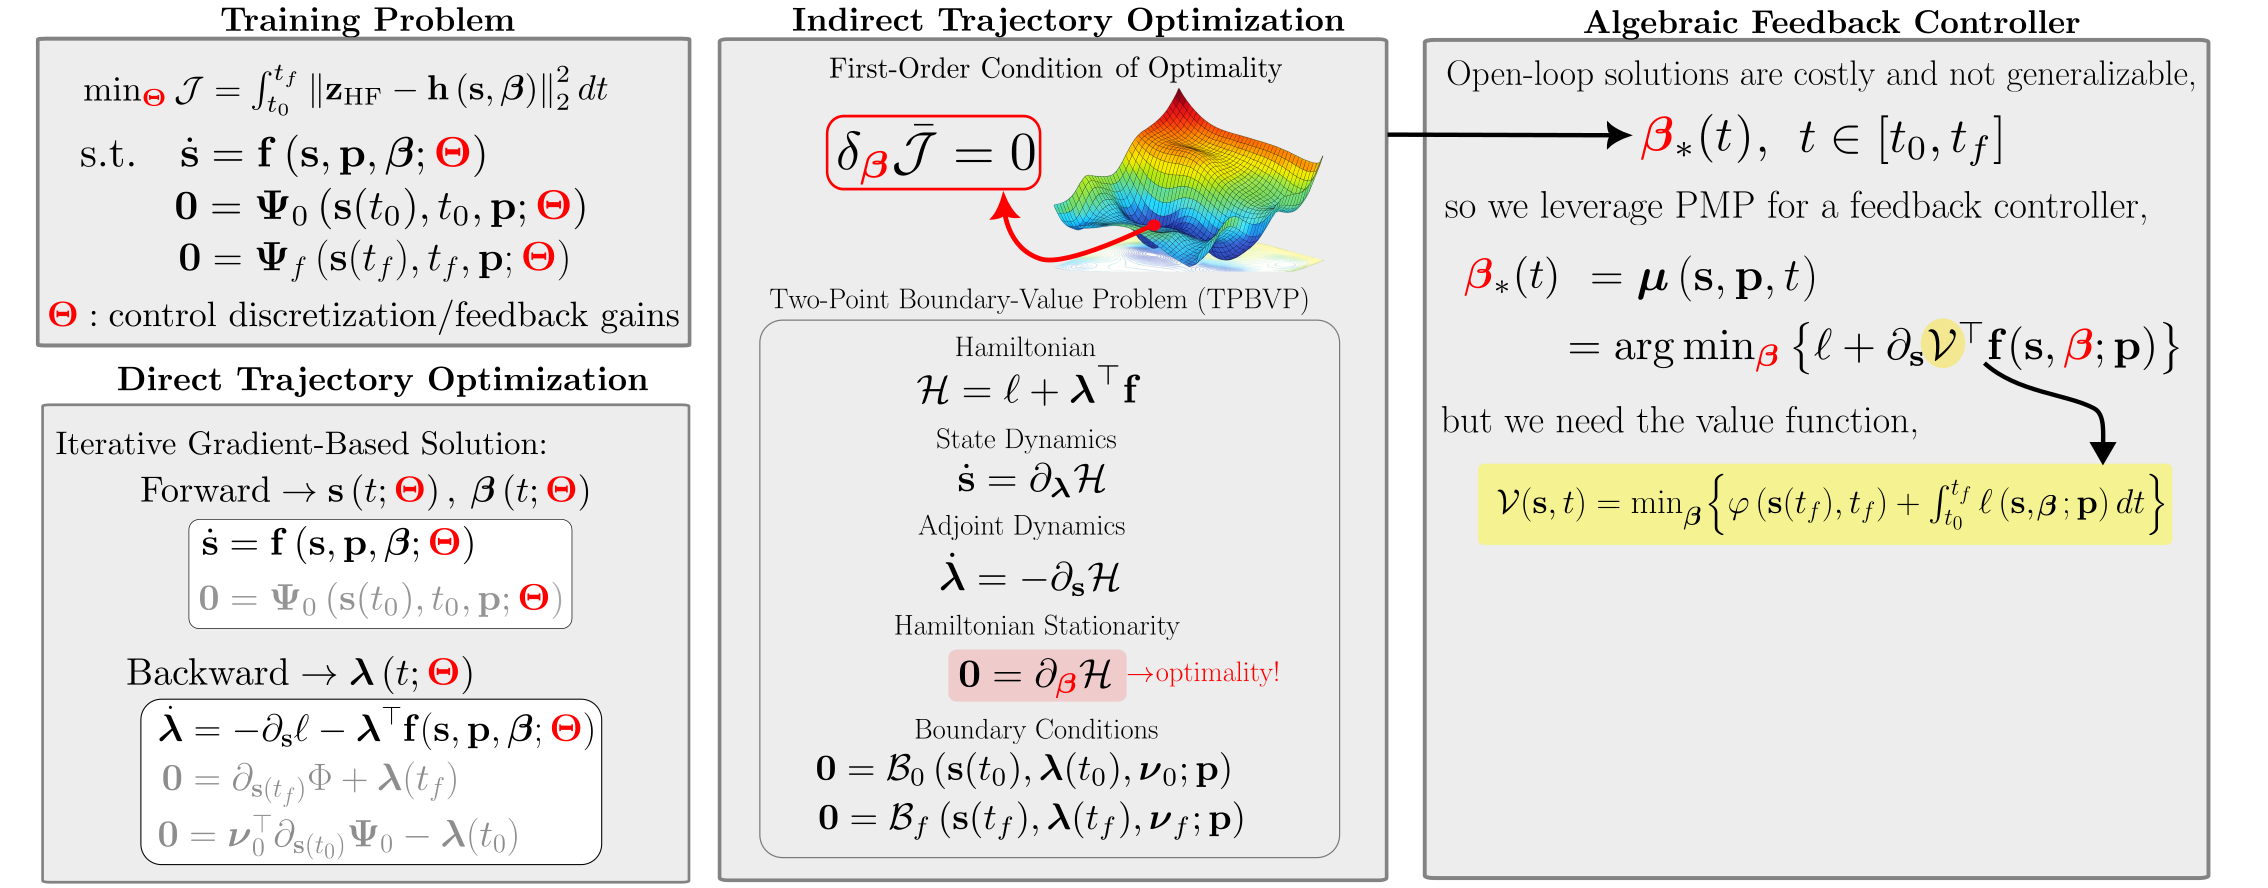
\includegraphics[width=0.95\textwidth]{../figs/ct/ct_overview_17.png}
        \end{figure}}
    \only<19>{
        \begin{figure}
            \centering
            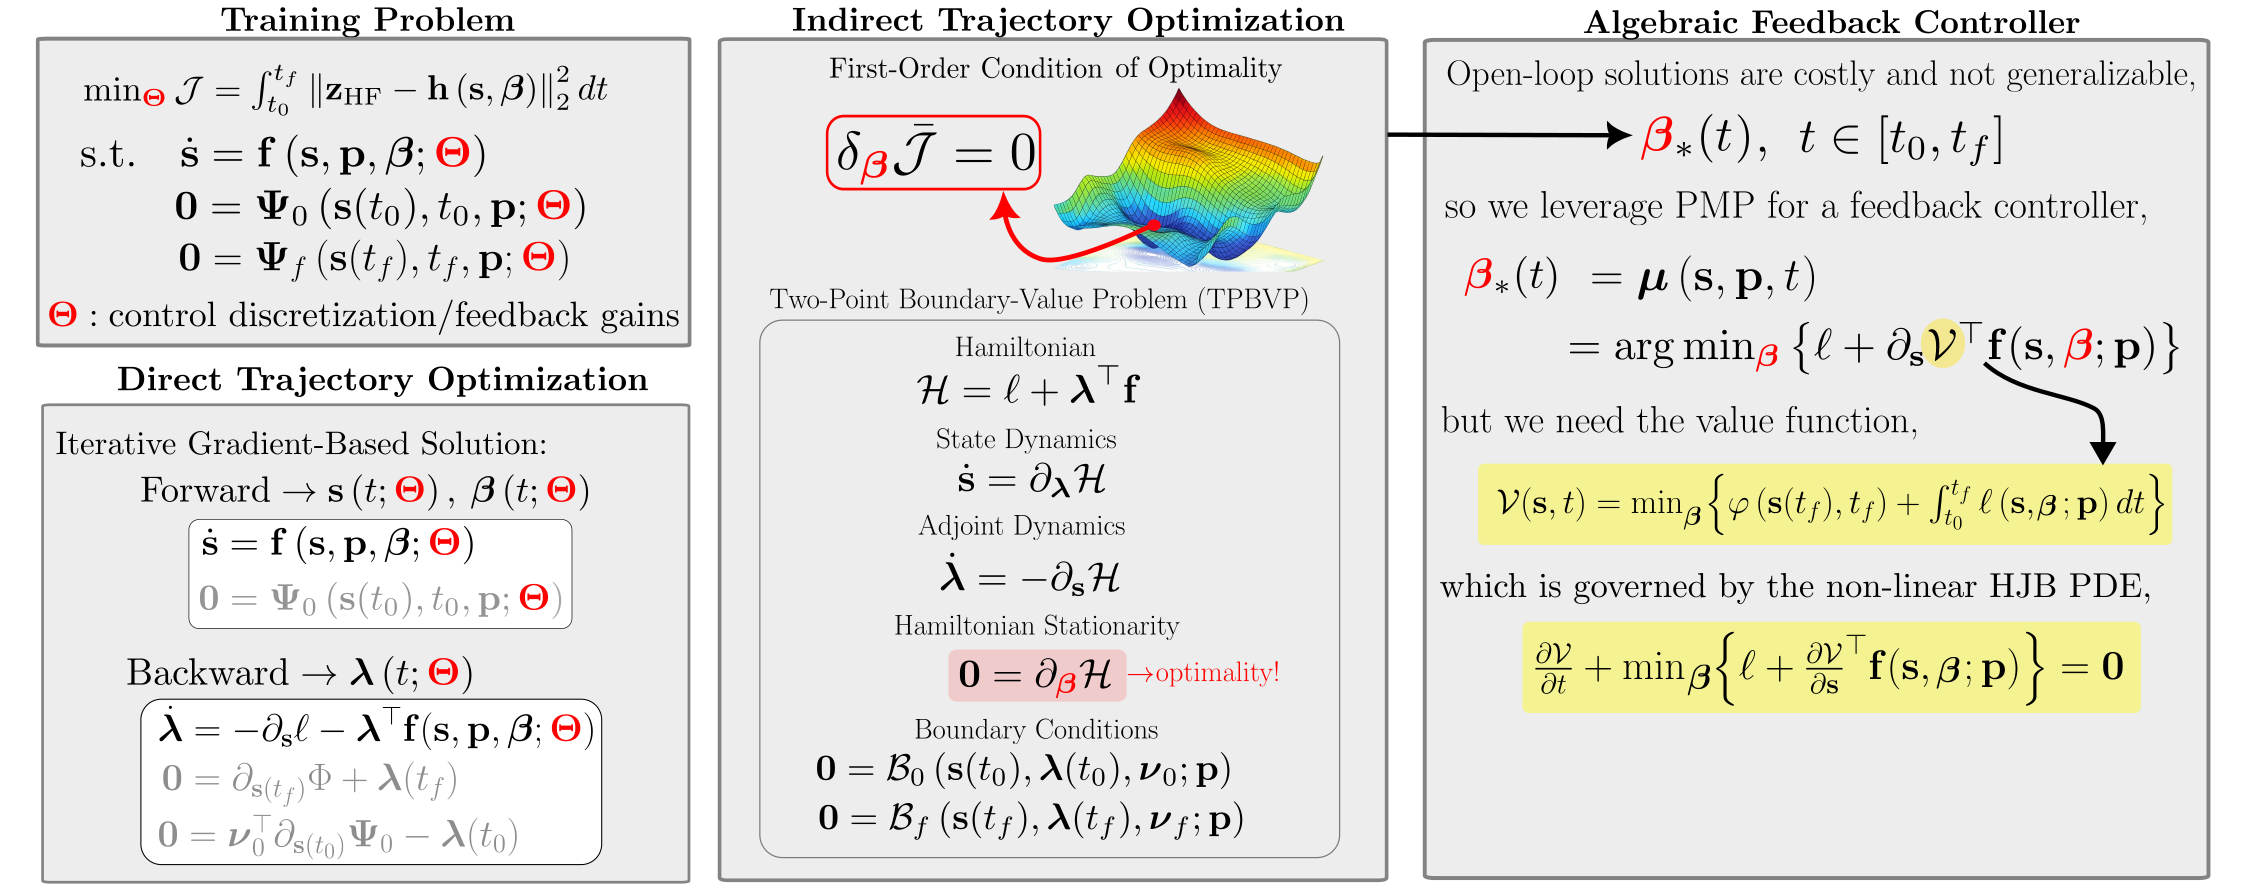
\includegraphics[width=0.95\textwidth]{../figs/ct/ct_overview_18.png}
        \end{figure}}
    \only<20>{
        \begin{figure}
            \centering
            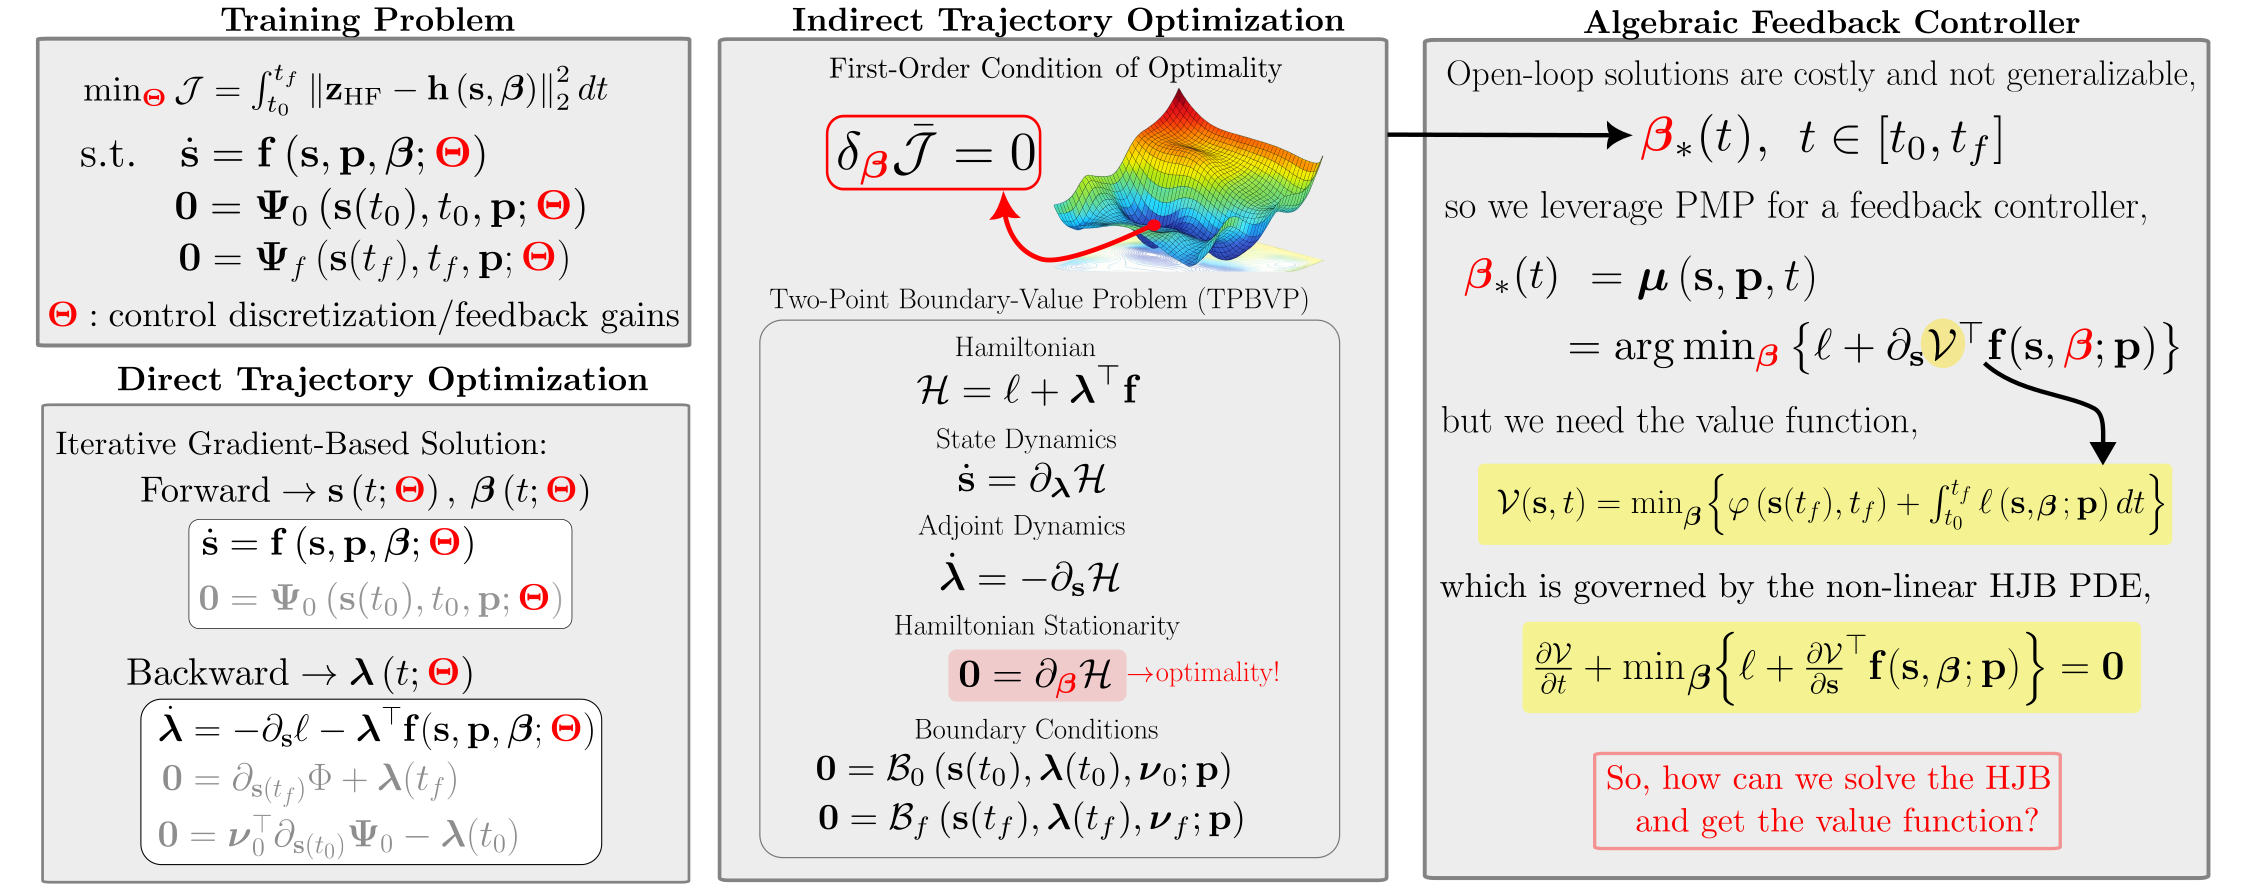
\includegraphics[width=0.95\textwidth]{../figs/ct/ct_overview_19.png}
        \end{figure}}
    \visible<2->{
    \begin{center}
        \vspace*{-0.1in}
        {\tiny
        $\vs$: state, $\Phi$: penalized terminal constraint, $\vbeta$: control action, $\cB_0,\cB_f$: boundary conditions, $\vnu$: Lagrange multipliers, $\vf$: non-linear dynamics, $\bar{\cJ}$: augmented cost functional, PMP: Pontryagin's Minimum Principle, HJB: Hamilton-Jacobi-Bellman
        }
    \end{center}}
\end{frame}
